\documentclass{kjpaper}
\usepackage[authoryear,sort&compress,round]{natbib}
\bibliographystyle{abbrvnat}
\usepackage{float}
\usetikzlibrary{positioning,arrows.meta,fit,backgrounds,calc}
\usepgfplotslibrary{groupplots,colormaps}
\pgfplotsset{discard if not/.style 2 args={y filter/.append code={%
  \edef\kjtempa{\thisrow{#1}}\edef\kjtempb{#2}\ifx\kjtempa\kjtempb\else\def\pgfmathresult{nan}\fi}},
  unbounded coords=discard}
% ---- project macros ----
\newcommand{\sname}{STRATA}
\newcommand{\code}[1]{\texttt{#1}}
\newcommand{\pgrad}{p_{\mathrm{grad}}}
\newcommand{\pdem}{p_{\mathrm{dem}}}
\newcommand{\pprune}{p_{\mathrm{prune}}}
\newcommand{\lhit}{l_{\mathrm{hit}}}
\newcommand{\lmiss}{l_{\mathrm{miss}}}
\newcommand{\amin}{a_{\min}}
\newcommand{\Nmin}{N_{\min}}
\title{\sname: One Geometry-Free Persistence-and-Periodicity Engine for Selectable 2D/3D Lifelong LiDAR Mapping}
\correspondingauthor{kangjmo91@gmail.com}
\paperurl{https://github.com/kjungmo/strata}
\author[1]{Jungmo Kang}
\affil[1]{Independent Researcher, Seoul, Republic of Korea}
\keywords{lifelong mapping, occupancy grids, voxel hashing, persistence filtering, FreMEn periodicity, ROS~2}
\begin{document}
\begin{abstract}
A robot that maps the same building for weeks cannot fold every LiDAR hit permanently into one grid: parked carts, passing people and doors that open on a schedule all burn in, and the map drifts toward a record of everything ever seen. Lifelong mapping must therefore keep walls (durability), forget movers (plasticity) and treat a cyclic door as signal rather than noise (periodicity), yet the systems that do this today embed that logic inside full lifelong-SLAM pipelines tied to one map geometry. We introduce \emph{\sname}, a small, SLAM-free persistence-and-periodicity engine that resolves the three requirements in one per-cell state machine---windowed log-odds with survival decay, a Schmitt-trigger graduation band, and a FreMEn-style incremental Fourier test---and drives a fixed-array 2D occupancy grid and an unbounded 3D voxel hash behind one interface selected by a single runtime string. The only per-backend code is the point-to-key map and the free-space ray walk; the classifier is shared by composition and builds as plain C++17 with Eigen, exercised by 32 unit tests. On a seeded synthetic suite, both backends graduate a static wall by the third window and hold recall 1.0 thereafter, with periodicity off or on. Removing hysteresis raises flicker from 54 to 574 toggles on identical noise, and memory stays at a flat 56~B per cell. Periodicity detection is the weak point. 50\%-duty doors are detected at true-positive rate 2/3 at every read-out length, but the false-positive rate on Bernoulli clutter varies from 0 to 4/5 with read-out length (2/5 at 64 windows, mean 0.331), and enabling periodicity raises total flicker on noisy walls by about half (5472 against 3672 toggles). We also correct a defect in the first release: its Fourier coefficients were not mean-removed, so a constant wall could be demoted from Static. Centring them keeps walls Static in every experiment and restores Static recall from 0 to 1 over the last 12 windows of the static-quality run. Evaluation is synthetic only. Code: \url{https://github.com/kjungmo/strata}.
\end{abstract}

\maketitle
\section{Introduction}\label{sec:intro}

\begin{figure}[t]
\centering
\resizebox{\linewidth}{!}{%
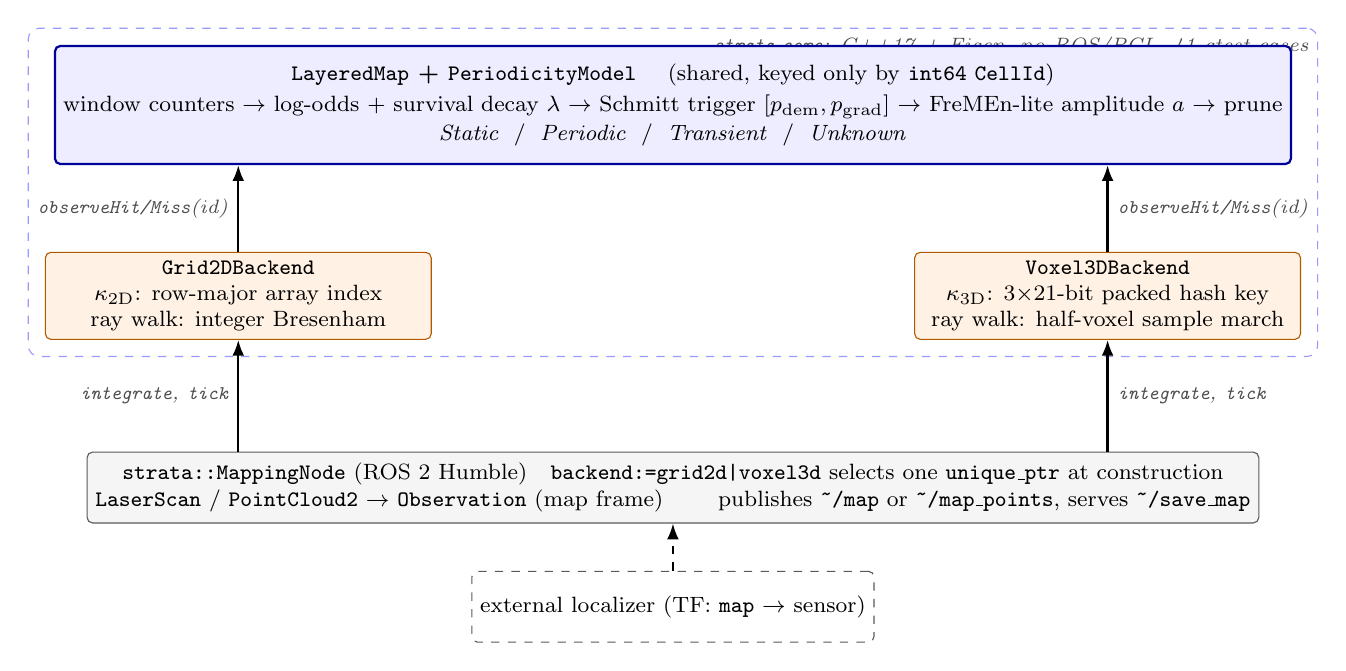
\begin{tikzpicture}[
  font=\footnotesize,
  box/.style={draw, rounded corners=2pt, align=center, minimum height=9mm, inner sep=3pt, fill=white},
  eng/.style={box, fill=blue!7, draw=blue!60!black, thick},
  geo/.style={box, fill=orange!10, draw=orange!70!black},
  ros/.style={box, fill=gray!8, draw=gray!70!black},
  arr/.style={-{Latex[length=2mm]}, thick},
  lab/.style={font=\scriptsize\itshape, text=black!70}]
% ---- engine (geometry-free) ----
\node[eng, minimum width=10.4cm, minimum height=15mm] (lm) at (0,0)
  {\textbf{\code{LayeredMap} + \code{PeriodicityModel}} \quad (shared, keyed only by \code{int64} \code{CellId})\\[2pt]
   window counters $\to$ log-odds $+$ survival decay $\lambda$ $\to$ Schmitt trigger $[\pdem,\pgrad]$ $\to$ FreMEn-lite amplitude $a$ $\to$ prune\\[1pt]
   \emph{Static} \;/\; \emph{Periodic} \;/\; \emph{Transient} \;/\; \emph{Unknown}};
% ---- backends ----
\node[geo, below left=11mm and -48mm of lm, minimum width=4.9cm] (g2)
  {\textbf{\code{Grid2DBackend}}\\ $\kappa_{2\mathrm{D}}$: row-major array index\\ ray walk: integer Bresenham};
\node[geo, below right=11mm and -48mm of lm, minimum width=4.9cm] (v3)
  {\textbf{\code{Voxel3DBackend}}\\ $\kappa_{3\mathrm{D}}$: 3$\times$21-bit packed hash key\\ ray walk: half-voxel sample march};
\draw[arr] (g2.north) -- node[lab, left] {\code{observeHit/Miss}(id)} (g2.north |- lm.south);
\draw[arr] (v3.north) -- node[lab, right] {\code{observeHit/Miss}(id)} (v3.north |- lm.south);
% band labels
\begin{scope}[on background layer]
\node[fit=(lm)(g2)(v3), draw=blue!40, dashed, rounded corners=4pt, inner sep=6pt,
  label={[lab, anchor=north east]north east:\code{strata\_core}: C++17 + Eigen, no ROS/PCL, 41 gtest cases}] (core) {};
\end{scope}
% ---- ROS node ----
\node[ros, below=12mm of core.south, minimum width=10.4cm] (node)
  {\textbf{\code{strata::MappingNode}} (ROS~2 Humble)\quad \code{backend:=grid2d|voxel3d} selects one \code{unique\_ptr} at construction\\
   \code{LaserScan} / \code{PointCloud2} $\to$ \code{Observation} (map frame) \qquad
   publishes \code{\textasciitilde/map} or \code{\textasciitilde/map\_points}, serves \code{\textasciitilde/save\_map}};
\draw[arr] (node.north -| g2.south) -- node[lab, left] {\code{integrate}, \code{tick}} (g2.south);
\draw[arr] (node.north -| v3.south) -- node[lab, right] {\code{integrate}, \code{tick}} (v3.south);
\node[ros, below=6mm of node, minimum width=4.2cm, fill=white, dashed] (tf) {external localizer (TF: \code{map} $\to$ sensor)};
\draw[arr, dashed] (tf) -- (node);
\end{tikzpicture}}
\caption{\textbf{Overview of \sname.} One geometry-free engine (top) owns every persistence and periodicity decision and sees only integer cell keys. The two backends (middle) contribute exactly two things: the point-to-key map $\kappa_b$ and the free-space ray walk. A thin ROS~2 node (bottom) selects one backend from a single string parameter and consumes, but never produces, the sensor pose.}
\label{fig:overview}
\end{figure}


An occupancy grid built the textbook way accumulates evidence and never lets go of it \citep{thrun2005probabilistic}. For a robot that drives a route once this is harmless; for one that maps the same warehouse or hospital corridor for weeks it is a slow failure. A cart parked for an afternoon, a person walking past and a load-bearing wall all leave the same kind of mark, and after enough passes the map describes the union of everything the sensor ever touched rather than the building. Lifelong mapping has to hold three requirements at once: the map must be \emph{durable} enough to keep structure that is genuinely permanent, \emph{plastic} enough to forget structure that has moved on, and it must do both without one global forgetting rate that is simultaneously too slow to erase movers and too fast to trust a wall---the stability--plasticity dilemma that \citet{biber2005dynamicmaps} framed for dynamic maps. A third requirement complicates the split: some structure is \emph{cyclic}, such as a door open every morning and shut every night. Its occupancy is a periodic temporal signal, and a flat decay law erases exactly the regularity that makes it predictable \citep{krajnik2017fremen,krajnik2014spectral}.

The systems that come closest to meeting all three are heavier than the problem requires. ELite \citep{gil2025elite} and LT-mapper \citep{kim2022ltmapper} resolve durability against plasticity, but as stages of full lifelong-SLAM pipelines with multi-session registration, place recognition and alignment. RTAB-Map \citep{labbe2019rtabmap} is the closest engineering precedent for selectable 2D and 3D geometry under one framework, and it too is a complete SLAM system with loop closure and memory tiering. Khronos \citep{schmid2024khronos} generalises the two-timescale idea to a metric-semantic scene graph. In each case the persistence-and-classification logic a robot needs is welded inside a larger apparatus and, usually, to one map geometry. What the surveyed prior art lacks is that piece on its own: a standalone, SLAM-free, dependency-light engine that performs only graduation, forgetting and periodicity labelling, runs under either 2D or 3D geometry, and can sit beneath an external localizer.

To overcome this coupling, we introduce \emph{\sname}, a persistence-and-periodicity engine whose cells carry temporal strata---Static, Periodic and Transient classes over an Unknown baseline---inside one per-cell state machine (Figure~\ref{fig:overview}). The state machine never sees coordinates. Both shipped backends translate world points into \code{int64} cell keys and walk a free-space ray to clear it; everything downstream of the key happens once, in the shared engine. Choosing 2D or 3D is one runtime string parameter resolved at construction, and the engine (\code{strata\_core}) links no ROS, DDS, TF or PCL, so its scientific logic builds and unit-tests without a ROS installation. We state the scope up front: \sname\ is not SLAM (it consumes an external \code{map}$\to$sensor transform), it models single-session persistence rather than multi-session remapping, and its evaluation is synthetic. Our contributions are:
\begin{itemize}
  \item \emph{One Geometry-Free Engine, Two Geometries}: a single \code{int64}-keyed engine (\code{LayeredMap} with \code{PeriodicityModel}) drives a fixed-array 2D grid and an unbounded 3D voxel hash through one \code{MapBackend} interface; the only per-backend code is the point-to-key map and the free-space ray walk (\S\ref{sec:method}), and the core builds with C++17 and Eigen alone under 41 behaviour-level tests.
  \item \emph{A Minimal Lifelong Classifier}: survival decay after the Persistence Filter \citep{rosen2016persistence}, a Schmitt-trigger graduation band motivated by Removert \citep{kim2020removert}, negative-evidence ray clearing as in ReFusion \citep{palazzolo2019refusion}, and a parallel FreMEn-lite periodicity test \citep{krajnik2017fremen} whose per-read-out false-alarm probability under iid clutter and occupancy-independent sampling is bounded for any noise rate by a Chernoff argument (Proposition~\ref{prop:chernoff}), emitting a four-class label from one SLAM-free module, with every equation transcribed from the shipped code and three implementation-versus-specification differences stated explicitly.
  \item \emph{A Mechanistic, Reproducible Characterisation}: a calibration run on held-out seeds (E0) and four seeded experiments (E1--E4) that isolate backend equivalence, periodicity detection, the contribution of hysteresis and decay, and per-dimension cost, with every table and figure regenerated from committed CSVs and failure modes diagnosed rather than averaged away.
\end{itemize}

Across the suite, both backends graduate a 161-cell wall by the third window and keep recall at 1.0 through window 39; their only quality gap, a final static precision of 0.9253 (\code{grid2d}) against 0.9758 (\code{voxel3d}) under 100 movers per window, arises in the backends' native sampling rather than in the shared classifier. We report and correct two defects of the first release's periodicity test, with before-and-after results. An uncentred Fourier amplitude could demote constant walls. An uncalibrated amplitude threshold labelled Bernoulli clutter Periodic at 0 to 4 of 5 cells depending on read-out length, a mean false-positive rate of 0.331 even after centring. With the calibrated test, the false-positive rate is 0 at every read-out length from 8 to 100 windows. Both 50\%-duty doors are still detected, for a true-positive rate of 2/3, but only from 15 windows instead of 8, and the one miss is a provable interaction between pruning and the amplitude gate. Removing the hysteresis band raises flicker from 54 to 574 toggles at the same decay, and the engine costs a flat 56~B per cell, with the 5.5--15.0$\times$ per-call gap between backends explained by 4.4--10.0$\times$ more live 3D cells. These results show that the lifelong-mapping core can be written once and shared across dimensions without a per-dimension cost of its own.

\section{Related Work}\label{sec:related}

\noindent\textbf{Lifelong and persistent mapping.} ELite \citep{gil2025elite} scores each point's ephemerality at two timescales and maintains a lifelong/static/delta map triad; LT-mapper \citep{kim2022ltmapper} composes live, meta and delta maps through explicit alignment, removal and graduation stages. Khronos \citep{schmid2024khronos} splits an active window from a long-term reconstruction with semantics, and \citet{yang2025lifelong3d} keep versioned deltas over a base map so that past sessions can be rebuilt. Classifying cells by their temporal behaviour predates these systems. Temporal occupancy grids \citep{arbuckle2002temporal} classify cells by occupancy over several timescales with planar laser range-finders and locate doors in a real-world setting; \citet{mitsou2007temporal} index every cell's occupancy history over time and separate static, low-dynamic and high-dynamic cells, in simulation with known poses. Multi-timescale and static/temporary map splits follow in \citet{biber2005dynamicmaps} and \citet{meyerdelius2010temporary}. \citet{pomerleau2014longterm} infer online whether each 3D point is static or dynamic from repeated observations, over seven months of data, and \citet{berrio2021longterm} report a long field deployment of a purge/promote pipeline. For 2D occupancy grids, \citet{stefanini2022efficient,stefanini2023safe} update a LiDAR occupancy map for long-term operation while accounting for localisation error, with the aim of keeping the map current rather than modelling periodic change. Two 2026 works, concurrent with this one, produce layered outputs: MTD-Map \citep{kim2026mtdmap} encodes the direction and duration of occupancy transitions per voxel in one stage and outputs static, dynamic and transition maps, evaluated on real datasets against established baselines, and \citet{chen2026layer} assign map content to long-term static, potentially dynamic and removed observed-dynamic layers from geometric and semantic evidence. Neither describes an explicit periodic class. \sname\ implements only the graduation half of this pattern---one per-cell state machine with no scan matching, loop closure, session alignment, semantics or object layer---and is intended as the core such systems wrap, not a competitor; correspondingly, it lacks their real-data and field-scale evidence.

\noindent\textbf{Persistence, forgetting and periodicity.} The Persistence Filter \citep{rosen2016persistence} estimates each feature's survival probability from a Bayesian survival-time model, and the Markov-chain occupancy models of \citet{tipaldi2013lifelong} and \citet{saarinen2012imac} learn per-cell transition rates. Perpetua \citep{saavedraruiz2025perpetua} combines persistence and emergence filters under multiple hypotheses for features that disappear and reappear. FreMEn \citep{krajnik2017fremen}, descending from spectral analysis of long-term maps \citep{krajnik2014spectral}, models cyclic occupancy with a few Fourier components selected by amplitude from a set of candidate periods, and it is the closest prior work to \sname. \citet{krajnik2016persistent} use it in a 2D spatio-temporal occupancy grid in which each cell represents both persistence (through the mean time between state changes) and periodicity; the grid integrates one map per patrol, replaces the ROS map server, and predicts time-specific maps for localisation and planning. FROctomap \citep{krajnik2014froctomap} applies the same model to 3D octree voxels, the exploration work of \citet{krajnik2015exploration} displays the static and daily-periodic cells of such a grid, and the open-source FreMEn repository \citep{fremenrepo} provides separate 2D-grid and octree packages, and also a generic server that maintains FreMEn models of arbitrary binary states keyed by an identifier. Warped hypertime \citep{krajnik2019warped} extends the idea to pseudo-periodic variation. \sname\ is narrower than this family in period modelling: it tests one configured base period and its harmonics and does not select periods. It differs from the family in two respects: its primary output is a discrete class, reached through a hysteresis band and pruning, rather than a predicted occupancy probability; and it attaches a finite-sample false-alarm bound to the periodic label. It also updates once per window, whereas the grid of \citet{krajnik2016persistent} integrates one map per patrol. \sname\ uses the log-odds update of \citet{thrun2005probabilistic}, clamped as in OctoMap \citep{hornung2013octomap}, replaces the survival posterior with one global multiplicative decay (a constant-rate special case), and runs a bounded FreMEn-style accumulator in parallel with graduation so that an oscillating cell is labelled Periodic instead of being mis-graduated or mis-pruned.

\noindent\textbf{Dynamic-object removal and negative evidence.} Removert \citep{kim2020removert} removes dynamic points conservatively and then reverts wrongly removed static ones; ERASOR \citep{lim2021erasor} removes them offline from pseudo-occupancy ratios; ReFusion \citep{palazzolo2019refusion} treats a reliably observed empty voxel as evidence. \sname\ applies the same logic online and per cell: a graduated cell demotes only after sustained contradicting evidence (a hysteresis band rather than a revert pass), and free-space misses along each ray are the evidence that demotes it.

\noindent\textbf{Map data structures and ROS~2 tooling.} OctoMap \citep{hornung2013octomap} and UFOMap \citep{duberg2020ufomap} share the clamped log-odds core but compress space with octrees, the latter with an explicit unknown state; the voxel hash of \citet{niessner2013hashing} is the structure \code{voxel3d} follows. Nav2's spatio-temporal voxel layer \citep{macenski2020stvl} decays costmap evidence for planning, layered costmaps \citep{lu2014layered} composite per-cell layers, and SLAM Toolbox \citep{macenski2021slamtoolbox} bounds lifelong 2D SLAM at the pose-graph level. For swappable backends, ROS~2 offers \code{pluginlib} \citep{ros2pluginlib}; \sname\ deliberately uses one interface and a two-way factory instead. Relative to the works above, the structural difference is narrow. Periodicity modelling that does not depend on geometry already exists, since the FreMEn server models any binary state that has an identifier \citep{fremenrepo}. What \sname\ shares, unchanged, between its 2D and 3D ray-casting backends is the full cell-level state machine: windowed log-odds with survival decay, graduation and demotion hysteresis, pruning, layer classification and the periodicity test.

\noindent\textbf{Periodicity tests and error control.} The periodic test uses the generalised Lomb--Scargle periodogram \citep{zechmeister2009gls}. Analytic false-alarm probabilities for periodogram peaks, including the search over frequencies, are derived under white Gaussian noise \citep{baluev2008}. For binary series, \citet{schmidtke2026binary} test a constant success probability against a periodic one of unspecified period, with a level that holds asymptotically. \sname\ addresses a narrower question: a finite-sample, distribution-free bound for independent Bernoulli occupancy at one configured period and its harmonics, under any sampling pattern fixed independently of the occupancy. Proposition~\ref{prop:chernoff} obtains it from the moment-generating-function bound for quadratic forms of sub-Gaussian vectors of \citet[Remark~2]{hsu2012tail}, followed by Markov's inequality and a union bound, with the variance proxy of Hoeffding's lemma \citep{hoeffding1963}; the result is an application of that bound, not a new inequality. Spending the level over the touch count (Proposition~\ref{prop:spend}) is a Bonferroni-type allocation over repeated looks, related to the alpha-spending functions of group-sequential trials \citep{lan1983discrete}; time-uniform bounds from nonnegative supermartingales \citep{howard2020timeuniform} are the modern alternative for repeated testing, which we do not use.

\section{\sname: A Geometry-Free Engine Beneath Two Map Geometries}\label{sec:method}

\sname\ is delivered as two ROS~2 packages with a hard dependency boundary. \code{strata\_core} holds the entire occupancy, persistence and periodicity logic together with both geometry backends, in C++17 with Eigen as its only third-party dependency. \code{strata} is a thin node that owns message conversion, TF lookups, publishers, a save service and file I/O (Appendix~\ref{app:io}). This section specifies the engine exactly as implemented: every equation is transcribed from \code{strata\_core}, and \S\ref{subsec:specdiff} lists where the code departs from the design document.

\noindent\textbf{Problem Setup: One Classifier, Any Geometry.} A sensor sweep at integration tick $k$ delivers an origin $\mathbf{o}_k\in\mathbb{R}^3$ and a set of hit endpoints $\mathcal{P}_k\subset\mathbb{R}^3$, both already in the map frame (the pose comes from an external localizer). A backend $b\in\{\mathrm{2D},\mathrm{3D}\}$ supplies two operators only: a key map $\kappa_b:\mathbb{R}^3\to\mathcal{C}\cup\{\bot\}$ onto integer cell ids $\mathcal{C}\subset\mathbb{Z}$, and a ray walk $\rho_b(\mathbf{o},\mathbf{p})\subset\mathcal{C}$ listing the free cells between origin and endpoint. Ticks are grouped into windows $w=1,2,\dots$. Each live cell $i$ carries a state $\mathbf{x}_i=(\ell_i,N_i,g_i,\boldsymbol{\phi}_i)$---log-odds occupancy, touched-window count, graduated flag and Fourier accumulators---and the map reads out a class $c_i\in\{\mathsf{U},\mathsf{T},\mathsf{P},\mathsf{S}\}$ (Unknown, Transient, Periodic, Static). The design objective is that the per-window map update factor as
\begin{equation}\label{eq:objective}
  \mathcal{X}_w=\Phi\big(\mathcal{X}_{w-1},\,\Gamma_b(\{(\mathbf{o}_k,\mathcal{P}_k)\}_{k\in w})\big),\qquad c_i=\Psi(\mathbf{x}_i),
\end{equation}
where only the evidence extractor $\Gamma_b$ depends on the backend, while the engine $\Phi$ and the read-out $\Psi$ are written once and see nothing but integer ids. The classes should make walls \emph{durable} ($\mathsf{S}$ persists under clutter), movers \emph{plastic} ($\mathsf{T}$ cells are forgotten), and cyclic structure \emph{periodic} ($\mathsf{P}$ is neither baked into $\mathsf{S}$ nor pruned). The stages below instantiate $\Gamma_b$, $\Phi$ and $\Psi$; Algorithm~\ref{alg:endwindow} gives the complete window update.

\subsection{Keying Observations: Reducing Geometry to Integer Cell Ids}\label{subsec:keying}

For every endpoint $\mathbf{p}\in\mathcal{P}_k$ the backend registers one miss on each cell of $\rho_b(\mathbf{o}_k,\mathbf{p})$ and then one hit on $\kappa_b(\mathbf{p})$. The engine keeps only per-window counters,
\begin{equation}\label{eq:gamma}
  h_{i,w}=\sum_{k\in w}\sum_{\mathbf{p}\in\mathcal{P}_k}\big[\kappa_b(\mathbf{p})=i\big],\qquad
  m_{i,w}=\sum_{k\in w}\sum_{\mathbf{p}\in\mathcal{P}_k}\big|\{j\in\rho_b(\mathbf{o}_k,\mathbf{p}) : j=i\}\big|,
\end{equation}
creating a cell lazily on first touch with $\ell_i=0$, $N_i=0$, $g_i=\text{false}$. This is $\Gamma_b$; it is the only backend-specific code.

\noindent\textbf{Fixed 2D grid.} \code{Grid2DBackend} addresses a $W\times H$ array with resolution $r$ and origin $(x_0,y_0)$, drops $z$, and maps a point to a row-major index,
\begin{equation}\label{eq:key2d}
  \kappa_{\mathrm{2D}}(\mathbf{p})=\Big\lfloor\tfrac{p_y-y_0}{r}\Big\rfloor W+\Big\lfloor\tfrac{p_x-x_0}{r}\Big\rfloor,
\end{equation}
returning $\bot$ (the hit is dropped) outside the array. $\rho_{\mathrm{2D}}$ is integer Bresenham \citep{bresenham1965} from the sensor cell up to but excluding the hit cell, so the sensor cell is included and the hit cell receives only its hit.

\noindent\textbf{Sparse 3D hash.} \code{Voxel3DBackend} floor-divides each axis by the voxel size $v$, offsets it by $2^{20}$ to keep it non-negative, and packs the three 21-bit fields into one 64-bit key,
\begin{equation}\label{eq:key3d}
  \kappa_{\mathrm{3D}}(\mathbf{p})=\big(u_x\ll 42\big)\,\big|\,\big(u_y\ll 21\big)\,\big|\,u_z,\qquad u_a=\lfloor p_a/v\rfloor+2^{20}.
\end{equation}
The map grows through the hash and needs no preallocated extent. Its key space is nevertheless finite: each 21-bit field represents the indices $-2^{20}$ to $2^{20}-1$ around the origin, far beyond the extent of a building at the default voxel size, and the code does not check this range, so a point outside it would receive a wrong key rather than being dropped. $\rho_{\mathrm{3D}}$ is a sample march rather than an exact voxel traversal: with $\mathbf{d}=\mathbf{p}-\mathbf{o}$ and $S=\lfloor\|\mathbf{d}\|/(v/2)\rfloor$ half-voxel steps, the interior samples $\mathbf{o}+s\,\mathbf{d}/\max(S,1)$, $s=1,\dots,S{-}1$, are hashed with \eqref{eq:key3d}. This is simpler than exact traversal but can visit a voxel more than once along a long ray and can skip a thin one when $S$ rounds down.

\subsection{Accumulating Evidence: Windowed Log-Odds with Survival Decay}\label{subsec:logodds}

A window closes on integration tick $k$ when $L\le 1$ or $k \bmod L=0$, with $L$ the \code{layer\_interval}. The ROS node can instead close windows every \code{window\_period\_s} seconds of message time (\code{window\_mode} \code{time}, the shipped setting; the code default and every experiment use $L$). A window that observes nothing changes no cell, so a silent gap of $k$ windows is exactly $k$ updates done in one pass; silent windows advance the phase without a touch, so within one uninterrupted stream of message time, and as long as message loss and TF drops are independent of occupancy, the false-alarm bound of \S\ref{subsec:fremen} holds in either mode and only the period, and with it the power, depends on the window rule. A bag loop or clock reset re-anchors only the clock while cell histories carry on, so neither the bound nor the persistence evidence holds across one; restart the node rather than loop a bag. Scan-counted windows last $L$ divided by the rate of messages actually integrated (\S\ref{sec:disc}). The update then scores every live cell once, so a single hit outweighs any number of misses in the same window:
\begin{equation}\label{eq:score}
  \tau_{i}=[h_{i,w}>0\lor m_{i,w}>0],\qquad o_{i}=[h_{i,w}>0],\qquad f_{i}=[h_{i,w}=0\land m_{i,w}>0].
\end{equation}
For \emph{touched} cells only ($\tau_i=1$), one log-odds increment is applied, multiplied by the survival decay $\lambda$, and clamped:
\begin{equation}\label{eq:logodds}
  \ell_i\leftarrow\min\!\Big(l_{\max},\max\!\big(l_{\min},\;\lambda\,(\ell_i+o_i\,\lhit+f_i\,\lmiss)\big)\Big),\qquad N_i\leftarrow N_i+1,
\end{equation}
with occupancy probability $p_i=\sigma(\ell_i)=1/(1+e^{-\ell_i})$. The update is the inverse-sensor-model rule of \citet{thrun2005probabilistic} with a constant-rate special case of the Persistence Filter's forgetting \citep{rosen2016persistence}. The order matters: the decay multiplies the \emph{already incremented} value, so the fresh evidence is itself attenuated in the same window.

\begin{proposition}[Saturation under repeated hits]\label{prop:fixedpoint}
If a cell is hit in every window, $0<\lambda<1$, $\lhit>0$ and $l_{\min}\le0<l_{\max}$, then $\ell_i$ converges monotonically from $0$ to $\min\!\big(l_{\max},\,\ell^\star\big)$ with $\ell^\star=\lambda\lhit/(1-\lambda)$.
\end{proposition}
\begin{proof}
Without the clamp the recursion is $\ell\mapsto\lambda(\ell+\lhit)$, an affine contraction with factor $\lambda$ and unique fixed point $\ell^\star$; from $\ell=0<\ell^\star$ the iterates increase monotonically towards it. The clamp is monotone and, since every iterate is non-negative and $l_{\min}\le0$, only the upper bound can bind, so the clamped iterates increase to $\min(l_{\max},\ell^\star)$.
\end{proof}
With the shipped defaults (Table~\ref{tab:params}; $\lambda{=}0.97$, $\lhit{=}0.85$) $\ell^\star\approx 27.5$, so the clamp binds at $l_{\max}{=}5$ and $p_{\max}=\sigma(5)\approx 0.9933$. The default thresholds $\pgrad{=}0.8$ and $\pprune{=}0.05$ correspond to $\ell\ge\ln 4\approx 1.386$ and $\ell<\ln(1/19)\approx-2.944$.

\subsection{Gating Graduation: A Schmitt Trigger Against Flicker}\label{subsec:schmitt}

After the log-odds step, $p_i$ and the periodicity amplitude $a_i$ (\S\ref{subsec:fremen}) are recomputed for \emph{every} cell, touched or not, and the graduated flag follows a two-sided Schmitt trigger with two periodicity guards, evaluated in this order:
\begin{align}
  \text{graduate:}\quad & \lnot g_i\land\lnot\pi_i\land p_i\ge\pgrad\land N_i\ge\Nmin \;\Rightarrow\; g_i\leftarrow\text{true},\label{eq:grad}\\
  \text{demote:}\quad & g_i\land\big(p_i\le\pdem\lor\pi_i\big)\;\Rightarrow\; g_i\leftarrow\text{false},\label{eq:demote}
\end{align}
where $\pi_i$ is the periodic predicate of \eqref{eq:periodic}. The interval $[\pdem,\pgrad]$ is the hysteresis band: through the occupancy disjunct $p_i\le\pdem$, a Static cell demotes only after sustained contradicting evidence, not after one contradicting window---the failure that Removert's revert pass repairs after the fact \citep{kim2020removert} is prevented online. The guard $\lnot\pi_i$ keeps a periodic cell out of the static map; the term $\lor\,\pi_i$ removes a Static cell that later reveals periodicity. That term lies outside the band and has no hysteresis of its own. It cannot, however, fire without contradicting evidence: with the centred amplitude of \S\ref{subsec:fremen}, $\pi_i$ requires a cell to have been observed free in a substantial share of its touched windows (Remark~\ref{rem:leak}), so a wall that is occupied whenever it is seen is never demoted by it. The predicate also requires the noise-calibrated significance of Proposition~\ref{prop:chernoff}, with its level spent over the touch count. A graduated cell is never pruned, so by Proposition~\ref{prop:spend} a wall whose occupancy is merely iid noise is demoted by this term at some point of the run with probability at most $\delta$. The term still acts in a single window when it does fire; E3 measures its cost in flicker with periodicity on (\S\ref{subsec:ablation}).

\begin{proposition}[No same-window oscillation]\label{prop:nooscillation}
If $\pdem<\pgrad$, a cell that graduates by \eqref{eq:grad} in a window is not demoted by \eqref{eq:demote} in the same window.
\end{proposition}
\begin{proof}
Graduation requires $\lnot\pi_i$ and $p_i\ge\pgrad>\pdem$, and $p_i,\pi_i$ are not recomputed between \eqref{eq:grad} and \eqref{eq:demote}, so both disjuncts of the demotion condition are false.
\end{proof}

\subsection{Detecting Periodicity: A FreMEn-Lite Amplitude Test}\label{subsec:fremen}

In parallel with occupancy, every touched cell feeds an incremental Fourier model following FreMEn \citep{krajnik2017fremen}. The model is restricted to one configured base period and its first harmonics; unlike FreMEn, it does not select periods from a candidate set, so a cycle whose frequency is not a harmonic of the base frequency is outside its scope. With window index $w$, base period $T$ (in windows), $H$ harmonics, $\omega=2\pi/\max(1,T)$, occupancy sample $o_i\in\{0,1\}$ and $\theta_k=(k{+}1)\omega w$, the accumulators $\boldsymbol{\phi}_i=(n_i,S_{0,i},C_{k,i},S_{k,i},E^{c}_{k,i},E^{s}_{k,i})$ evolve as
\begin{equation}\label{eq:gather}
  n_i\mathrel{+}=1,\quad S_{0,i}\mathrel{+}=o_i,\quad C_{k,i}\mathrel{+}=o_i\cos\theta_k,\quad S_{k,i}\mathrel{+}=o_i\sin\theta_k,\quad E^{c}_{k,i}\mathrel{+}=\cos\theta_k,\quad E^{s}_{k,i}\mathrel{+}=\sin\theta_k,
\end{equation}
for $k=0,\dots,H{-}1$. Here $n_i$ counts \emph{touched} windows, not elapsed ones, and $E^{c},E^{s}$ record the phases at which the cell was touched. With the touched-window mean $\bar{o}_i=S_{0,i}/n_i$, the \emph{centred} coefficients are $\alpha_k=2(C_{k,i}-\bar{o}_iE^{c}_{k,i})/n_i$ and $\beta_k=2(S_{k,i}-\bar{o}_iE^{s}_{k,i})/n_i$, i.e.\ $\alpha_k+\mathrm{i}\beta_k=\tfrac{2}{n_i}\sum_{w\in\mathcal{W}_i}(o_{i,w}-\bar{o}_i)\,e^{\mathrm{i}\theta_k}$ over the touched windows $\mathcal{W}_i$, the mean-removed spectrum of FreMEn. The harmonic amplitudes and the dominant amplitude are
\begin{equation}\label{eq:amp}
  a_{i,k}=\sqrt{\alpha_k^2+\beta_k^2},\qquad
  a_i=\begin{cases}0, & n_i<T,\\ \max_{0\le k<H}a_{i,k}, & n_i\ge T,\end{cases}
\end{equation}
and the periodic predicate $\pi_i$, which adds a significance test to the amplitude threshold, is given in \eqref{eq:periodic} below.
The phase prediction $\hat{p}_i(w)=\mathrm{clip}_{[0,1]}\big(S_{0,i}/n_i+\sum_k[\alpha_k\cos((k{+}1)\omega w)+\beta_k\sin((k{+}1)\omega w)]\big)$ is exposed for downstream use. The gate $n_i\ge T$ withholds a harmonic estimate until a period's worth of touches exists; a sparsely observed cell needs $T$ \emph{touches}, which can span many more than $T$ windows.

\begin{remark}[Centring, and the defect it corrects]\label{rem:leak}
Centring bounds the amplitude by the occupancy variation. Since $|o_{i,w}-\bar{o}_i|$ averages $2\bar{o}_i(1-\bar{o}_i)$ over $\mathcal{W}_i$, the triangle inequality gives
\[
  a_i\;\le\;4\,\bar{o}_i(1-\bar{o}_i)
\]
under any sampling of $\mathcal{W}_i$. A cell that is occupied (or free) in every touched window therefore has $a_i=0$, and $\pi_i$ with $\amin{=}0.3$ requires $0.081<\bar{o}_i<0.919$: at least about 8\% of its touched windows must be free. The code as first released (v0.1.0) omitted $E^{c},E^{s}$, so its coefficients were uncentred. For an always-occupied cell, $a_i$ was then twice the mean phase vector of $\mathcal{W}_i$: it measured \emph{when} the cell was observed, not how its occupancy varied. For $n$ consecutive touches this is
\[
  a_i=\max_{0\le k<H}\frac{2\,\big|\sin\big(n(k{+}1)\pi/T\big)\big|}{n\,\big|\sin\big((k{+}1)\pi/T\big)\big|}\;\le\;\frac{2}{n\sin(\pi/T)}.
\]
It exceeds $\amin$ at $n=10$--$13$ for $T{=}8$ (peak 0.439 at $n{=}11$; the bound clears only from $n{=}18$), and at $n=29$--$40$ for the shipped $T{=}24$, $H{=}2$ (bound: $n\ge52$). Through the $\lor\,\pi_i$ term of \eqref{eq:demote}, whose predicate was then $a_i\ge\amin$ alone, a wall hit every window therefore left the Static layer for 120 integration ticks at $L{=}10$. Uneven phase coverage made this permanent: a wall seen in 8 of every 48 windows had $a_i\approx1.66$. The corrected engine adds the two phase sums, 16 bytes per harmonic (the significance test below adds two more), and the per-cell cost order is unchanged. Ten regression tests cover both failures and genuine detection; seven of them fail on v0.1.0 and all pass after the fix (\S\ref{subsec:setup}), and Table~\ref{tab:fix} compares E1--E3 before and after.
\end{remark}

\noindent\textbf{Calibrating the Periodic Test Against Noise.} Centring removes the bias of the amplitude but not its variance, and $a_i\ge\amin$ alone is not a test. If a cell's occupancy is pure noise, $o_{i,w}\sim\mathrm{Bernoulli}(m)$ independently of the phase, each centred coefficient has variance $2m(1{-}m)/n_i$ under uniform phase coverage, a standard deviation of $\sqrt{0.5/8}=0.25$ at $m{=}\tfrac12$, $n_i{=}T{=}8$. A fixed $\amin$ is then crossed by chance at short lengths, and pruning (\S\ref{subsec:classify}) keeps returning cells to short lengths. We therefore test each harmonic for significance. Write $c_w=\cos\theta_k$, $s_w=\sin\theta_k$ over the touched windows, $\tilde{\mathbf{z}}_w=(c_w-\bar c,\,s_w-\bar s)^{\top}$ for the centred phase vectors, $\mathbf{y}_{i,k}=\sum_{w\in\mathcal{W}_i}(o_{i,w}-\bar o_i)\,\tilde{\mathbf{z}}_w=\tfrac{n_i}{2}(\alpha_k,\beta_k)^{\top}$ and $\mathbf{M}_{i,k}=\sum_{w}\tilde{\mathbf{z}}_w\tilde{\mathbf{z}}_w^{\top}$. Then
\begin{equation}\label{eq:dchi}
  d_{i,k}=\mathbf{y}_{i,k}^{\top}\mathbf{M}_{i,k}^{-1}\mathbf{y}_{i,k},\qquad B(r)=\begin{cases}2r\,e^{1-2r}, & r>\tfrac12,\\ 1, & r\le\tfrac12,\end{cases}
\end{equation}
where $d_{i,k}$ is the drop in squared residual when a sinusoid at harmonic $k$ is fitted with a floating mean, the generalised Lomb--Scargle periodogram \citep{zechmeister2009gls}. $\mathbf{M}_{i,k}$ needs two more accumulators per harmonic, $\sum\cos2\theta_k$ and $\sum\sin2\theta_k$, since $\sum c_w^2=\tfrac12(n_i+\sum\cos2\theta_k)$ and $\sum c_ws_w=\tfrac12\sum\sin2\theta_k$. The periodic predicate requires, for some harmonic, both an effect size and significance at a nominal level $\delta$ (\code{periodic\_false\_alarm}):
\begin{equation}\label{eq:periodic}
  \pi_i=\texttt{enable\_periodicity}\land n_i\ge T\land\exists k:\ \big[a_{i,k}\ge\amin\ \land\ H\,B(d_{i,k})\le\delta\big].
\end{equation}
Proposition~\ref{prop:chernoff} bounds the false-alarm probability of this predicate. It is an application of known results, not a new inequality: the moment-generating-function step is the bound of \citet[Remark~2]{hsu2012tail} for a quadratic form of a sub-Gaussian vector, here with the identity matrix and Hoeffding's variance proxy $\tfrac14$, and the rest is Markov's inequality and a union bound over the harmonics. We state it with the explicit constants that the shipped test uses.

\begin{proposition}[Calibrated false-alarm bound]\label{prop:chernoff}
Let the touched windows $\mathcal{W}_i$ ($|\mathcal{W}_i|=n$) be fixed independently of the occupancy, and let $o_{i,w}$, $w\in\mathcal{W}_i$, be independent $\mathrm{Bernoulli}(m)$ for one unknown $m\in[0,1]$. If $\mathbf{M}_{i,k}$ is non-singular, then $\Pr(d_{i,k}\ge r)\le B(r)$ for every $r>0$. Consequently, for every $\amin\ge0$ and $0<\delta<H$, the predicate \eqref{eq:periodic} is true with probability at most $\delta$.
\end{proposition}
\begin{proof}
Because $\sum_w\tilde{\mathbf{z}}_w=\mathbf{0}$, the unknown mean drops out: $\mathbf{y}_{i,k}=\sum_w\xi_w\tilde{\mathbf{z}}_w$ with $\xi_w=o_{i,w}-m$. Put $\mathbf{b}_w=\mathbf{M}_{i,k}^{-1/2}\tilde{\mathbf{z}}_w$ and $\mathbf{u}=\sum_w\xi_w\mathbf{b}_w$, so that $d_{i,k}=\|\mathbf{u}\|^2$ and $\sum_w\mathbf{b}_w\mathbf{b}_w^{\top}=\mathbf{I}_2$. Each $\xi_w$ has mean zero and lies in an interval of length 1, so Hoeffding's lemma \citep{hoeffding1963} gives $\mathbb{E}\,e^{t\xi_w}\le e^{t^2/8}$, and by independence $\mathbb{E}\,e^{\mathbf{v}^{\top}\mathbf{u}}\le\exp\big(\tfrac18\sum_w(\mathbf{v}^{\top}\mathbf{b}_w)^2\big)=e^{\|\mathbf{v}\|^2/8}$ for every $\mathbf{v}\in\mathbb{R}^2$. Following \citet{hsu2012tail}, let $\mathbf{g}\sim\mathcal{N}(\mathbf{0},\mathbf{I}_2)$ be independent of $\mathbf{u}$. For $0\le\eta<2$, $\mathbb{E}_{\mathbf{g}}\,e^{\sqrt{2\eta}\,\mathbf{g}^{\top}\mathbf{u}}=e^{\eta\|\mathbf{u}\|^2}$, so exchanging the expectations,
\[
  \mathbb{E}\,e^{\eta d_{i,k}}=\mathbb{E}_{\mathbf{g}}\,\mathbb{E}_{\mathbf{u}}\,e^{\sqrt{2\eta}\,\mathbf{g}^{\top}\mathbf{u}}\le\mathbb{E}_{\mathbf{g}}\,e^{\eta\|\mathbf{g}\|^2/4}=(1-\eta/2)^{-1}.
\]
Markov's inequality gives $\Pr(d_{i,k}\ge r)\le(1-\eta/2)^{-1}e^{-\eta r}$, and $\eta=2-1/r$ (admissible for $r>\tfrac12$) yields $2r\,e^{1-2r}$; for $r\le\tfrac12$ the bound 1 is trivial. $B$ decreases strictly from 1 to 0 on $(\tfrac12,\infty)$, so $H\,B(d_{i,k})\le\delta$ holds exactly when $d_{i,k}\ge r^\star$ with $B(r^\star)=\delta/H$. The union bound over the $H$ harmonics then gives $\Pr(\pi_i)\le H\cdot\delta/H=\delta$.
\end{proof}
The bound needs no knowledge of $m$: the sub-Gaussian constant $\tfrac14$ is the Bernoulli worst case $m=\tfrac12$. When $\mathbf{M}_{i,k}$ is singular (for instance at a Nyquist harmonic), the code projects onto its range; the same argument with a one-dimensional $\mathbf{g}$ gives the smaller bound $(1-\eta/2)^{-1/2}e^{-\eta r}$, so $B$ stays valid. Under uniform phase coverage at a harmonic with $2(k{+}1)\not\equiv0\pmod T$ (so that the sine column does not vanish; the defaults $T/H\in\{8/3,24/2\}$ satisfy it) $\mathbf{M}_{i,k}=\tfrac{n}{2}\mathbf{I}_2$ and $d_{i,k}=n\,a_{i,k}^2/2$, so \eqref{eq:periodic} becomes an amplitude threshold that shrinks with $n$,
\begin{equation}\label{eq:astar}
  a_{i,k}\ \ge\ \max\big(\amin,\ a^\star(n)\big),\qquad a^\star(n)=\sqrt{2r^\star/n}.
\end{equation}
For $\delta{=}0.1$ and $H{=}3$, $r^\star=3.115$, so $a^\star(8)=0.883$ and $a^\star(64)=0.312$. The bound is conservative: in the Gaussian limit at $m{=}\tfrac12$, $\Pr(d_{i,k}\ge r)\to e^{-2r}$, a factor $2e\,r$ below $B(r)$, or about 17 at $r^\star$. We therefore first treated $\delta$ as a nominal level for one read-out and chose it on a calibration set disjoint from every evaluation seed (E0, \S\ref{subsec:setup}). The pre-stated rule took the largest $\delta\in\{0.01,0.02,0.05,0.1,0.2\}$ whose measured per-read-out false-alarm rate stays at or below 0.01, both over a null grid and in the live pipeline, and it selected $\delta{=}0.1$ (Table~\ref{tab:e0}). That rule compares point estimates: the worst pipeline rate at $\delta{=}0.1$, 7 of 1000 cells, has a 95\% Wilson upper limit of 0.0144 \citep{wilson1927}, so the calibration does not establish the 0.01 target with confidence. Only $\delta$ is held out; the test itself was introduced after the amplitude-only rule produced false positives on the E2 seed, so E2 is not a blind evaluation of its design. More importantly, one read-out is not what the map does.

\noindent\textbf{Spending the Level Over Repeated Read-Outs.} The map evaluates \eqref{eq:periodic} after every window, so a clutter cell gets one chance per read-out, and pruning \eqref{eq:prune} erases its history and starts another. E5 measures the consequence: at a single-read-out level of 0.1, up to 953 of 2000 Bernoulli clutter cells are labelled Periodic at some window within 1024 windows (\S\ref{subsec:traj}). The shipped rule therefore replaces the constant level $\delta$ in \eqref{eq:periodic} by a level that decreases with the touch count,
\begin{equation}\label{eq:spend}
  \delta_n=\delta\,\frac{T}{n(n+1)}\quad(n\ge T),\qquad \sum_{n\ge T}\delta_n=\delta ,
\end{equation}
where the sum telescopes because $T/(n(n{+}1))=T/n-T/(n{+}1)$. This is a Bonferroni-type allocation of the level over the sequence of read-outs, in the spirit of the alpha-spending functions used for repeated significance tests in group-sequential trials \citep{lan1983discrete}; Proposition~\ref{prop:spend} is the union bound over it.

\begin{proposition}[Trajectory-level false-alarm bound]\label{prop:spend}
Call a \emph{history} of cell $i$ its touched windows from its creation until it is pruned or the run ends. Suppose that, given everything observed before the history begins, its touched windows are fixed independently of its occupancy and its occupancy samples are independent $\mathrm{Bernoulli}(m)$. With the level $\delta_n$ of \eqref{eq:spend} in \eqref{eq:periodic}, the probability that $\pi_i$ holds at some read-out of the history is at most $\delta$, whatever the length of the run. If $L_N$ histories of the cell begin in windows $1,\dots,N$, the probability that the cell is labelled Periodic at some window up to $N$ is at most $\delta\,\mathbb{E}[L_N]$.
\end{proposition}
\begin{proof}
Condition on everything observed before the history begins; under the hypothesis the history is then a fixed-design sample. For $n\ge T$ let $D_n$ be the event that the statistic of its first $n$ samples, computed as if the cell were never pruned, satisfies \eqref{eq:periodic} at level $\delta_n$. Proposition~\ref{prop:chernoff} with $\delta_n$ in place of $\delta$ gives $\Pr(D_n)\le\delta_n$. A read-out at touch count $n$ evaluates $\pi_i$ on exactly these $n$ samples (read-outs between two touches repeat the last value), and it happens only if the history survived to $n$, so the event that $\pi_i$ ever holds is contained in $\bigcup_{n\ge T}D_n$. The union bound gives at most $\sum_{n\ge T}\delta_n=\delta$; pruning only removes read-outs. For the second claim, the $\ell$-th history begins at a window determined by the past, so the probability that it begins by $N$ and fires is at most $\delta$ times the probability that it begins by $N$; summing over $\ell$ gives $\delta\,\mathbb{E}[L_N]$.
\end{proof}
The proposition is strongest where pruning does not act. A graduated cell is exempt from \eqref{eq:prune}, so a Static wall has one history and the probability that the $\lor\,\pi_i$ term of \eqref{eq:demote} ever demotes it on iid noise is at most $\delta$ for the whole run. For clutter that is pruned and re-created, the bound grows with the number of histories, which depends on the data: a Bernoulli(0.4) cell under the E2 parameters begins about 62 histories in 1024 windows, and $\delta\,\mathbb{E}[L_N]$ is then vacuous. That regime is measured (E5), not guaranteed. The null is still that of Proposition~\ref{prop:chernoff}: temporally correlated clutter violates it, and E5 shows that the test flags such clutter. The shipped level is chosen on separate calibration seeds, now at trajectory level. The pre-stated rule takes the largest $\delta\in\{0.01,0.02,0.05,0.1,0.2\}$ for which the rate of ever labelling a Bernoulli clutter cell Periodic within 1024 windows has a Wilson 95\% upper limit \citep{wilson1927} of at most 0.01 in every calibration configuration. It selects $\delta{=}0.2$, the largest candidate (Table~\ref{tab:e5choice}), and this is the shipped default. For the shipped rule, then, what is proved is the per-history bound 0.2; the 0.01 target is a measurement. Under uniform coverage the threshold of \eqref{eq:astar} becomes $a^\star(n)=\sqrt{2r^\star_n/n}$ with $B(r^\star_n)=\delta_n/H$, which falls roughly like $\sqrt{\log n/n}$ rather than $1/\sqrt n$. The detection delay is the price: in E2 a 50\%-duty door with $T{=}8$ is detected from 25 windows, against 15 with a single-read-out level of 0.1 and 8 without the test.

\subsection{Classifying and Pruning: Four Classes from One State}\label{subsec:classify}

At the end of the same per-cell pass, a cell with little evidence is erased together with its Fourier accumulators:
\begin{equation}\label{eq:prune}
  \text{erase } i \iff \lnot g_i\land p_i<\pprune\land a_i<\amin .
\end{equation}
Static cells and periodic cells are therefore never pruned. The guard uses the lenient effect-size screen $a_i<\amin$ rather than $\lnot\pi_i$, so a \emph{candidate} periodic cell keeps its accumulators, and hence its growing $n_i$, until the test resolves it. Every other erased cell loses $\boldsymbol{\phi}_i$. We considered keeping the Fourier history of erased cells and rejected it: pruning exists so that clutter does not accumulate, and a record for every cell ever touched would grow without bound, fastest in \code{voxel3d}, where every sampled free voxel is a cell. A re-created cell restarts at $n_i=0$ with a new history and, under \eqref{eq:spend}, a new level budget; this is why the trajectory bound of Proposition~\ref{prop:spend} scales with the number of histories. The read-out $\Psi$ of \eqref{eq:objective} is a priority ladder,
\begin{equation}\label{eq:classify}
  c_i=\begin{cases}
    \mathsf{U} & i\text{ absent},\\
    \mathsf{S} & g_i,\\
    \mathsf{P} & \pi_i,\\
    \mathsf{T} & p_i\ge\pprune,\\
    \mathsf{U} & \text{otherwise},
  \end{cases}
\end{equation}
evaluated top to bottom. The node renders it with the convention Unknown $-1$, free 0, Transient 50, Periodic 75, Static 100, writing in ascending priority so Static wins any tie: \code{grid2d} keeps one byte per cell outside the classifier, an observed-free bit set by the ray clear and never cleared, a bit for a hit in the open window and a bit for whether the cell's last observation was a hit; it draws 50 for a cell hit in the open window or last observed as a hit, or a Transient cell whose evidence leans occupied ($p_i>0.5$), and 0 for a cleared cell last observed free, so free means last observed free; \code{voxel3d} publishes only Static voxel centres. The full transition table is in Appendix~\ref{app:io}. The update touches all $N$ live cells, including untouched ones, because \eqref{eq:grad}--\eqref{eq:prune} read the recomputed $p_i$ and $a_i$; its cost is $O(NH)$ per window, and between window closes a sweep costs $O(1)$ per endpoint plus the ray walk. Per-cell state is a 24-byte record plus roughly 32 bytes of hash-node overhead, the ${\sim}56$~B/cell used in \S\ref{sec:exp}. That figure is an estimate for the periodicity-off path, not a measurement. A Fourier record, with two scalar accumulators and six heap-allocated vectors of $H$ values in a second hash map, is allocated only for cells touched with periodicity enabled and is not included in it, nor are the hash tables' bucket arrays or the \code{grid2d} flag byte per grid cell with its list of cells touched in the open window.

\begin{algorithm}[t]
\caption{\code{endWindow}: one layered update per closed window, as in \code{layered\_map.cpp}}\label{alg:endwindow}
\KwIn{live cells $\mathcal{X}$ with window counters $h_i,m_i$; window index $w$}
$w\gets w+1$\;
\ForEach{live cell $i$}{
  $\tau\gets[h_i{>}0\lor m_i{>}0]$, $o\gets[h_i{>}0]$, $f\gets[h_i{=}0\land m_i{>}0]$\tcp*{Eq.~\eqref{eq:score}}
  \If{$\tau$}{
    $\ell_i\gets\mathrm{clamp}\big(\lambda(\ell_i+o\,\lhit+f\,\lmiss),\,l_{\min},\,l_{\max}\big)$, $N_i\gets N_i+1$\tcp*{Eq.~\eqref{eq:logodds}}
    \lIf{\code{enable\_periodicity}}{update $\boldsymbol{\phi}_i$ with $(o,w)$\tcp*[f]{Eq.~\eqref{eq:gather}}}
  }
  $p_i\gets\sigma(\ell_i)$, $a_i\gets\mathrm{amplitude}(\boldsymbol{\phi}_i)$, $\pi_i\gets$ Eq.~\eqref{eq:periodic} on $\boldsymbol{\phi}_i$\tcp*{Eqs.~\eqref{eq:amp}--\eqref{eq:periodic}}
  \lIf{$\lnot g_i\land\lnot\pi_i\land p_i\ge\pgrad\land N_i\ge\Nmin$}{$g_i\gets\text{true}$\tcp*[f]{Eq.~\eqref{eq:grad}}}
  \lIf{$g_i\land(p_i\le\pdem\lor\pi_i)$}{$g_i\gets\text{false}$\tcp*[f]{Eq.~\eqref{eq:demote}}}
  $h_i\gets0$, $m_i\gets0$\;
  \lIf{$\lnot g_i\land p_i<\pprune\land a_i<\amin$}{erase $i$ and $\boldsymbol{\phi}_i$\tcp*[f]{Eq.~\eqref{eq:prune}}}
}
\KwOut{updated $\mathcal{X}$; classes by Eq.~\eqref{eq:classify} on demand}
\end{algorithm}

\subsection{Selecting a Backend: One Interface, One String}\label{subsec:select}

\code{MapBackend} exposes four methods: \code{integrate(obs, origin)} runs $\Gamma_b$ for one sweep, \code{tick()} advances the integration counter and may close a window, and two read-only counters report Static and Transient cells. The node reads one string parameter, \code{backend} $\in\{$\code{grid2d}, \code{voxel3d}$\}$, holds one \code{unique\_ptr} per concrete backend and instantiates exactly one at construction; all engine parameters are read through one shared helper, so the tuning surface is backend-independent by construction. At two backends a runtime \code{dlopen} registry such as \code{pluginlib} \citep{ros2pluginlib} would add discovery machinery whose cost is not yet repaid. Because $\Phi$ and $\Psi$ in \eqref{eq:objective} never see coordinates, any behavioural or cost difference between the backends must originate in $\kappa_b$, $\rho_b$ or their input sampling---the property the experiments test.

\subsection{Reconciling Code and Specification}\label{subsec:specdiff}

We document the code that ships. Two places diverge from the design document (\code{SPEC.md}), and each changes operational semantics.

\begin{remark}[Forgetting is coupled to re-observation]\label{rem:fov}
The design document states that every cell decays every window. In the code, \eqref{eq:logodds} runs only for touched cells, so a cell outside the sensor's field of view neither decays nor relaxes toward the prior: its $\ell_i$ freezes. Clutter fades only while it is re-observed as free, and anything that leaves the field of view persists (\S\ref{sec:disc}).
\end{remark}
\begin{remark}[The amplitude gate counts touches]
The design document gates the amplitude on \emph{elapsed} windows; the code gates on the touched-window count $n_i$ of \eqref{eq:periodic}. This is the mechanism behind the low-duty-cycle miss in \S\ref{subsec:main}.
\end{remark}

\section{Experiments}\label{sec:exp}

We ask three questions. Do the two backends behave as one engine wearing two geometries (E1, E4)? Does the shared classifier detect periodic structure, and how does it fail (E2)? Which mechanism actually stabilises the static layer (E3)?

\subsection{Experimental Setup}\label{subsec:setup}

\noindent\textbf{Harness and protocol.} All four experiments are driven by a standalone harness that compiles directly against the \code{strata\_core} sources, with no ROS~2, ament or colcon in the loop; it lives in \nolinkurl{paper/experiments/}. One command, \nolinkurl{bash paper/experiments/run_all.sh}, builds the core and its unit tests, checks the \code{ctest} suite (one target aggregating the 32 gtest cases, ten of them regression tests for the amplitude defect of Remark~\ref{rem:leak}), builds and runs the four executables, and writes the CSVs in \nolinkurl{paper/experiments/results/}; every table and plot in this paper is regenerated from those files (Appendix~\ref{app:repro}). Every stochastic experiment derives its \code{std::mt19937} generator from the constant seed 12345 plus a per-run offset recorded in code, and the seed is logged in each CSV. All magnitudes are therefore single-seed point estimates: we report no cross-seed dispersion, and gaps such as 0.9253 against 0.9758 illustrate a mechanism rather than a distributional estimate.

\noindent\textbf{What is compared.} There is no external baseline: none of the related systems (\S\ref{sec:related}) exposes a SLAM-free, ROS-free persistence core that could be driven by the same harness, so a single-number comparison would not be like for like. Instead E1 and E4 compare the two \sname\ backends, each driven in its native geometry by its own seeded stream (\code{grid2d} on the integer lattice, \code{voxel3d} continuously); because both call the identical engine, any divergence arises in $\kappa_b$, $\rho_b$ or their input sampling. E2 and E3 drive \code{LayeredMap} directly with no backend at all, which by \eqref{eq:objective} characterises the classifier for whichever backend supplies the ids. Each harness sets its own parameters in code (Table~\ref{tab:eparams}); in particular all four run with one window per tick ($L{=}1$), so \emph{window} and \emph{frame} coincide.

\noindent\textbf{Metrics.} Static-set precision, recall and F1 against a known wall set (E1, E3); Periodic-class true- and false-positive rates against ground truth and the dominant amplitude $a$ (E2); \emph{flicker}, the number of per-window toggles of a wall cell's Static flag (E3); mean latency per \code{integrate()} call, cell updates per second in \code{endWindow()}, final live-cell count and estimated memory at 56~B per cell (E4).

\noindent\textbf{Scenarios and hardware.} E1: a 161-cell static cross (the segments $y{=}60$ and $x{=}60$ over $[20,100]$) hit every window, plus 5, 25 or 100 fresh random movers per window, for 40 windows, on a $120{\times}120$ grid and a voxel map, both at resolution 1.0, once with periodicity off and once with it on at the shipped $T{=}24$, $H{=}2$. E2: three periodic doors (period 8 at 4-on/4-off and 2-on/6-off, period 4 at 2-on/2-off), a constant wall and four Bernoulli(0.5) aperiodic controls, with $T{=}8$, $H{=}3$, read out at 64 windows and, in a sweep, after every length $n=8$--$100$ (a fresh map per length). E3: 50 wall cells observed occupied with probability 0.6 per window among 10 movers per window, 80 windows, the same noise replayed for all 36 configurations of $\pgrad\in\{0.6,0.7,0.8,0.9\}\times\pdem\in\{0.3,0.5,\pgrad\}\times\lambda\in\{0.90,0.97,1.0\}$, with periodicity off and again with it on at the shipped defaults. All results are from the corrected engine; the same harness run against the v0.1.0 engine is kept for comparison (Table~\ref{tab:fix}). E4: 150 random hits per window for 20 windows at nominal extents $100^2$, $250^2$ and $500^2$, resolution 1.0, periodicity off. E4 alone reads the wall clock; its absolute microseconds come from one machine whose specification is not recorded in the committed artifacts and are not claimed to be portable, whereas its live-cell counts follow only from ray geometry and are deterministic.

\subsection{Main Results}\label{subsec:main}

% AUTO-GENERATED by tools/make_artifacts.py from paper/experiments/results/e1_static_quality.csv -- do not edit
\begin{table}[t]
\centering
\caption{Static-layer quality (E1) against the 161-cell ground-truth wall set. \emph{Recall~1 from} is the first window index $t$ at which recall reaches 1.0 (it never drops afterwards); precision, F1 and the predicted static-set size are at the final window $t{=}39$. Single seed (12345), so no dispersion is reported. Bold marks the better backend under high clutter.}
\label{tab:e1}
\small
\begin{tabular}{llcccc}
\toprule
Backend & Clutter (movers/window) & Recall 1 from & Precision & F1 & $|\hat{\mathcal{S}}|$ \\
\midrule
\texttt{grid2d} & low (5) & $t{=}2$ & 1.0000 & 1.0000 & 161 \\
\texttt{grid2d} & med (25) & $t{=}2$ & 0.9938 & 0.9969 & 162 \\
\texttt{grid2d} & high (100) & $t{=}2$ & 0.9253 & 0.9612 & 174 \\
\midrule
\texttt{voxel3d} & low (5) & $t{=}2$ & 1.0000 & 1.0000 & 161 \\
\texttt{voxel3d} & med (25) & $t{=}2$ & 0.9938 & 0.9969 & 162 \\
\texttt{voxel3d} & high (100) & $t{=}2$ & \textbf{0.9758} & \textbf{0.9877} & 165 \\
\bottomrule
\end{tabular}
\end{table}

\begin{figure}[t]
\centering
\begin{tikzpicture}
\begin{groupplot}[group style={group size=2 by 1, horizontal sep=14mm},
  width=0.47\linewidth, height=0.32\linewidth, xmin=0, xmax=39, ymin=0.93, ymax=1.005,
  xlabel={window $t$}, grid=major, grid style={gray!20}, tick label style={font=\scriptsize},
  label style={font=\small}, title style={font=\small},
  legend style={font=\scriptsize, at={(0.97,0.03)}, anchor=south east}, legend cell align=left,
  restrict y to domain=0.9:1.1, unbounded coords=discard]
\nextgroupplot[title={\code{grid2d}}, ylabel={static-set F1}]
\addplot[thick, blue!70!black] table[x=window,y=f1] {figures/data/e1_grid2d_low.dat};
\addplot[thick, orange!80!black, dashed] table[x=window,y=f1] {figures/data/e1_grid2d_med.dat};
\addplot[thick, red!70!black, densely dotted] table[x=window,y=f1] {figures/data/e1_grid2d_high.dat};
\legend{low (5/w), med (25/w), high (100/w)}
\nextgroupplot[title={\code{voxel3d}}]
\addplot[thick, blue!70!black] table[x=window,y=f1] {figures/data/e1_voxel3d_low.dat};
\addplot[thick, orange!80!black, dashed] table[x=window,y=f1] {figures/data/e1_voxel3d_med.dat};
\addplot[thick, red!70!black, densely dotted] table[x=window,y=f1] {figures/data/e1_voxel3d_high.dat};
\end{groupplot}
\end{tikzpicture}
\caption{\textbf{Static-layer F1 over time (E1).} F1 is 0 for $t<2$ (no cell has met $\Nmin{=}3$; not shown) and reaches 1.0 at $t{=}2$ for every backend and clutter level. Only the 100-movers-per-window regime accumulates false statics, more so on \code{grid2d}. Plotted directly from \code{e1\_static\_quality.csv}.}
\label{fig:e1}
\end{figure}


\noindent\textbf{Backend equivalence of the static layer (E1).} With $\Nmin{=}3$ a cell needs three touched windows before it may graduate, and recall jumps from 0 to 1.0 exactly at the third window ($t{=}2$) for all six backend--clutter combinations, then holds at 1.0 through $t{=}39$: clutter never demotes a wall cell (Table~\ref{tab:e1}, Figure~\ref{fig:e1}). Table~\ref{tab:e1} is the periodicity-off run. With periodicity on at the shipped $T{=}24$, $H{=}2$ the run is identical window for window: the wall is occupied whenever it is touched, so its centred amplitude is 0 (Remark~\ref{rem:leak}). The v0.1.0 engine instead lost the whole wall from the Static layer in windows 29--40 ($t=28$--$39$), in all six runs, and ended with Static recall 0 (Table~\ref{tab:fix}). The only errors are false Static cells created when a random mover re-hits one cell often enough to graduate on its own. At 5 movers per window this never happens and precision stays at 1.0; at 25 it saturates at one spurious cell (precision 0.9938); at 100 false statics keep accumulating, from the first extra cell at $t{=}17$ (\code{grid2d}) or $t{=}25$ (\code{voxel3d}) to 174 or 165 predicted cells at $t{=}39$. This yields the one material gap between backends, precision 0.9253 against 0.9758. Both runs apply the identical graduation rule, each to its own natively sampled mover stream (movers on the integer lattice for \code{grid2d}, continuous for \code{voxel3d}, both confined to one $z$-plane), so the gap reflects quantisation and sampling rather than the classifier; we do not claim it isolates a single geometric mechanism.

% AUTO-GENERATED by tools/make_artifacts.py from paper/experiments/results/e2_classification.csv, e2_summary.csv -- do not edit
\begin{table}[t]
\centering
\caption{Periodicity detection (E2) after 64 windows, $a_{\min}{=}0.3$, $T{=}8$, $H{=}3$. \emph{Ref.\ amplitude} is a non-pruning reference model fed the identical occupancy stream. Periodic TPR $=2/3$, FPR $=1/5$.}
\label{tab:e2}
\small
\begin{tabular}{lcccc}
\toprule
Probe cell & Ground truth & Final class & Ref.\ amplitude & Outcome \\
\midrule
\texttt{door\_p8\_4on4off} (50\% duty) & periodic & Periodic & 0.653 & correct \\
\texttt{door\_p8\_2on6off} (25\% duty) & periodic & Transient & 0.462 & \textbf{miss} \\
\texttt{door\_p4\_2on2off} (50\% duty) & periodic & Periodic & 0.707 & correct \\
\texttt{wall\_constant} & non-periodic & Static & $\approx 0$ & correct \\
\texttt{aperiodic\_0} & non-periodic & Transient & 0.159 & correct \\
\texttt{aperiodic\_1} & non-periodic & Periodic & 0.329 & \textbf{false pos.} \\
\texttt{aperiodic\_2} & non-periodic & Transient & 0.139 & correct \\
\texttt{aperiodic\_3} & non-periodic & Transient & 0.251 & correct \\
\bottomrule
\end{tabular}
\end{table}

\begin{figure}[t]
\centering
\begin{tikzpicture}
\begin{axis}[width=0.82\linewidth, height=0.40\linewidth, xmode=log, log basis x=2,
  xtick={6,8,12,16,24,32,48,64}, xticklabels={6,8,12,16,24,32,48,64},
  xmin=5.5, xmax=70, ymin=-0.02, ymax=0.92,
  xlabel={observation length $n$ (touched windows)}, ylabel={dominant amplitude $a$},
  grid=major, grid style={gray!20}, tick label style={font=\scriptsize}, label style={font=\small},
  legend style={font=\scriptsize, at={(1.02,0.5)}, anchor=west}, legend cell align=left]
\addplot[thick, blue!70!black, mark=*, mark size=1.2pt] table[x=len,y=amp] {figures/data/e2_door_p8_4on4off.dat};
\addplot[thick, blue!40, mark=square*, mark size=1.2pt] table[x=len,y=amp] {figures/data/e2_door_p4_2on2off.dat};
\addplot[thick, teal!70!black, dashed, mark=triangle*, mark size=1.4pt] table[x=len,y=amp] {figures/data/e2_door_p8_2on6off.dat};
\addplot[thick, black, mark=x] table[x=len,y=amp] {figures/data/e2_wall_constant.dat};
\addplot[red!70!black, thick, densely dotted, mark=o, mark size=1.2pt] table[x=len,y=amp] {figures/data/e2_aperiodic_1.dat};
\addplot[gray, thin, mark=none] table[x=len,y=amp] {figures/data/e2_aperiodic_0.dat};
\addplot[gray, thin, mark=none, forget plot] table[x=len,y=amp] {figures/data/e2_aperiodic_2.dat};
\addplot[gray, thin, mark=none, forget plot] table[x=len,y=amp] {figures/data/e2_aperiodic_3.dat};
\addplot[red, thick, dashed, domain=5.5:70, samples=2, forget plot] {0.3};
\addplot[red!60!black, thick, dotted, forget plot] table[x=len,y=astar] {figures/data/e2_threshold.dat};
\node[font=\scriptsize, anchor=south west, text=red!60!black] at (axis cs:9,0.80) {$a^\star(n)$};
\draw[gray!70, dashed] (axis cs:8,-0.02) -- (axis cs:8,0.92);
\node[font=\scriptsize, anchor=south west, text=red] at (axis cs:40,0.30) {$\amin{=}0.3$};
\node[font=\scriptsize, anchor=north west, text=gray] at (axis cs:8,0.9) {$n{=}T$};
\legend{door p8 4/4, door p4 2/2, door p8 2/6, wall, aperiodic 1, aperiodic 0/2/3}
\end{axis}
\end{tikzpicture}
\caption{\textbf{FreMEn-lite amplitude against observation length (E2)}, from a non-pruning reference model of the corrected engine fed each probe cell's occupancy stream ($T{=}8$, $H{=}3$). The $n\ge T$ gate forces $a{=}0$ at $n{=}6$; both 50\%-duty doors settle well above $\amin$, and the 25\%-duty door would too, yet the live pipeline prunes it first (Proposition~\ref{prop:race}). The constant wall is exactly 0 at every length because the coefficients are centred (Remark~\ref{rem:leak}); the Bernoulli controls hover near $\amin$. The dotted curve $a^\star(n)$ is the amplitude the calibrated test of Proposition~\ref{prop:chernoff} requires at $\delta{=}0.1$, $H{=}3$ under uniform phase coverage (Eq.~\eqref{eq:astar}); a cell is Periodic only above both curves. Plotted from \code{e2\_amplitude\_vs\_length.csv}.}
\label{fig:e2}
\end{figure}

\begin{figure}[t]
\centering
\begin{tikzpicture}
\begin{axis}[name=fpr, width=0.82\linewidth, height=0.32\linewidth,
  xmin=7, xmax=101, ymin=-0.03, ymax=0.85, xtick={8,16,24,32,40,48,56,64,72,80,88,96},
  xticklabels={}, ylabel={Periodic FPR (of 5)},
  grid=major, grid style={gray!20}, tick label style={font=\scriptsize}, label style={font=\small},
  legend style={font=\scriptsize, at={(0.5,1.03)}, anchor=south, legend columns=3}, legend cell align=left]
\addplot[const plot, thick, gray, densely dashed] table[x=len,y=fpr] {figures/data/e2_fpr_pre.dat};
\addplot[const plot, thick, orange!80!black] table[x=len,y=fpr] {figures/data/e2_fpr_mid.dat};
\addplot[const plot, thick, violet!70!black] table[x=len,y=fpr] {figures/data/e2_fpr_one.dat};
\addplot[const plot, very thick, blue!70!black] table[x=len,y=fpr] {figures/data/e2_fpr_post.dat};
\addplot[const plot, thin, violet!70!black, densely dotted] table[x=len,y=reffpr] {figures/data/e2_fpr_one.dat};
\addplot[const plot, thin, blue!70!black, densely dotted] table[x=len,y=reffpr] {figures/data/e2_fpr_post.dat};
\draw[gray!70, dashed] (axis cs:64,-0.03) -- (axis cs:64,0.85);
\legend{v0.1.0, centred, single read-out, spent, single (no pruning), spent (no pruning)}
\end{axis}
\begin{axis}[at={(fpr.south west)}, anchor=north west, yshift=-4pt,
  width=0.82\linewidth, height=0.24\linewidth,
  xmin=7, xmax=101, ymin=-0.05, ymax=1.05, xtick={8,16,24,32,40,48,56,64,72,80,88,96},
  ytick={0,0.333,0.667,1}, yticklabels={0,1/3,2/3,1},
  xlabel={read-out length $n$ (windows)}, ylabel={TPR (of 3)},
  grid=major, grid style={gray!20}, tick label style={font=\scriptsize}, label style={font=\small}]
\addplot[const plot, thick, gray, densely dashed] table[x=len,y=tpr] {figures/data/e2_fpr_pre.dat};
\addplot[const plot, thick, orange!80!black] table[x=len,y=tpr] {figures/data/e2_fpr_mid.dat};
\addplot[const plot, thick, violet!70!black] table[x=len,y=tpr] {figures/data/e2_fpr_one.dat};
\addplot[const plot, very thick, blue!70!black] table[x=len,y=tpr] {figures/data/e2_fpr_post.dat};
\addplot[const plot, thin, blue!70!black, densely dotted] table[x=len,y=reftpr] {figures/data/e2_fpr_post.dat};
\draw[gray!70, dashed] (axis cs:64,-0.05) -- (axis cs:64,1.05);
\end{axis}
\end{tikzpicture}
\caption{\textbf{Periodic false- and true-positive rates against read-out length (E2)}, from the real \code{LayeredMap}, a fresh map per length, $T{=}8$, $H{=}3$, $\amin{=}0.3$, for the four engine versions of Table~\ref{tab:fix}. The dotted lines apply the single-read-out and the spent predicate to a non-pruning reference model fed the same streams (lower panel: spent only). The dashed vertical marks the $n{=}64$ read-out of Table~\ref{tab:e2}. The v0.1.0 and centred TPR curves coincide at 2/3. Plotted from \code{e2\_rates\_vs\_length.csv} and its three archived counterparts.}
\label{fig:e2fpr}
\end{figure}

% AUTO-GENERATED by tools/make_artifacts.py from paper/experiments/results/e1_static_quality{,_periodic}.csv, e2_summary.csv, e2_rates_vs_length.csv, e3_sensitivity{,_periodic}.csv, pre_fix_2026-09-28/, pre_calibration_2026-09-28/ and pre_spending_2026-09-28/ -- do not edit
\begin{table}[t]
\centering
\caption{Effect of the three corrections to the periodicity test, same harness, seeds and parameters. \emph{v0.1.0}: uncentred amplitude and the amplitude-only rule $a\ge\amin$ (results in \nolinkurl{results/pre\_fix\_2026-09-28/}); \emph{Centred}: centred amplitude, amplitude-only rule (\nolinkurl{results/pre\_calibration\_2026-09-28/}); \emph{Single}: the significance test of Proposition~\ref{prop:chernoff} at $\delta{=}0.1$ at every read-out (\nolinkurl{results/pre\_spending\_2026-09-28/}); \emph{Spent}: the level $\delta{=}0.2$ spent over the touch count (Proposition~\ref{prop:spend}, current engine). E1 and E3 with periodicity on use the shipped $T{=}24$, $H{=}2$, $\amin{=}0.3$; E2 uses $T{=}8$, $H{=}3$. E1 counts are identical in all six backend--clutter runs.}
\label{tab:fix}
\footnotesize
\setlength{\tabcolsep}{4pt}
\begin{tabular}{lccccc}
\toprule
& Periodicity & \multicolumn{4}{c}{Periodicity on} \\
\cmidrule(lr){3-6}
Measure & off & v0.1.0 & Centred & Single & Spent \\
\midrule
E1: windows $t\ge3$ with Static recall $<1$ & 0 windows & 12 ($t{=}28$--$39$) & 0 windows & 0 windows & 0 windows \\
E1: Static recall at $t{=}39$ & 1 & 0 & 1 & 1 & 1 \\
\midrule
E2 at $n{=}64$: TPR / FPR & -- & 2/3 / 1/5 & 2/3 / 2/5 & 2/3 / 0/5 & 2/3 / 0/5 \\
E2, $n=8$--$100$: mean FPR & -- & 0.363 & 0.331 & 0.000 & 0.000 \\
E2, $n=8$--$100$: FP count range (of 5) & -- & 0--4 & 0--4 & 0--0 & 0--0 \\
E2, $n=8$--$100$: lengths with no FP & -- & 10 of 93 & 7 of 93 & 93 of 93 & 93 of 93 \\
E2, $n=8$--$100$: lengths with constant wall Periodic & -- & 4 of 93 & 0 of 93 & 0 of 93 & 0 of 93 \\
E2, $n=8$--$100$: mean TPR & -- & 0.667 & 0.667 & 0.624 & 0.563 \\
E2: TPR 2/3 at every $n\ge$ & -- & 8 & 8 & 15 & 25 \\
E2, $n=8$--$100$: lengths with FP, no pruning & -- & -- & -- & 25 of 93 & 0 of 93 \\
\midrule
E3: total flicker, 36 configurations & 3672 & 7132 & 5472 & 3792 & 3672 \\
E3: flicker at $\pgrad{=}0.9$, $\pdem{=}0.3$, $\lambda{=}0.90$ & 54 & 138 & 102 & 58 & 54 \\
E3: flicker at $\pgrad{=}\pdem{=}0.9$, $\lambda{=}0.90$ & 574 & 582 & 596 & 576 & 574 \\
\bottomrule
\end{tabular}
\end{table}


\noindent\textbf{Periodicity detection (E2).} Both 50\%-duty doors are classified Periodic with amplitudes 0.653 and 0.707, well above $\amin{=}0.3$ (Table~\ref{tab:e2}). The constant wall is Static with amplitude exactly 0 at every length, and two of the four aperiodic controls end Transient. At the $n{=}64$ read-out the Periodic class therefore reaches a true-positive rate of 2/3 and a false-positive rate of 2/5. The v0.1.0 engine scored 1/5 at this length, so the corrected engine is \emph{worse} at the read-out previously reported, and we do not treat either value as representative. Figure~\ref{fig:e2fpr} reads the pipeline out at every length from 8 to 100. The true-positive rate is 2/3 at every length both before and after the fix, but the false-positive count ranges over 0--4 of 5 in both versions, with a mean false-positive rate of 0.363 before the fix and 0.331 after. The fix removes the constant wall from that count (it was Periodic at 4 of 93 lengths, now none). The remaining false positives are Bernoulli controls, and centring cannot suppress them because they genuinely vary. Two effects combine. First, $\amin{=}0.3$ is not calibrated against sampling noise: for a Bernoulli(0.5) cell observed $n$ times each centred coefficient has standard deviation $\sqrt{0.5/n}$, which is 0.25 at $n{=}T{=}8$. Second, pruning resets $\boldsymbol{\phi}_i$, so the live pipeline often estimates the amplitude from only the touches since a cell's last re-creation. At $n{=}64$, \code{aperiodic\_0} has reference amplitude 0.159 over all 64 windows but is Periodic in the pipeline, while \code{aperiodic\_1} has reference amplitude 0.329, 0.029 above $\amin$. A significance-calibrated threshold is future work (\S\ref{sec:disc}). The amplitude curves confirm the gate of \eqref{eq:periodic}: for the 4-on/4-off door the amplitude is exactly 0 at $n{=}6<T$, 0.653 at every sampled multiple of $T$ ($n=8,16,\dots,64$) and 0.581 at $n{=}12$, where the uncentred v0.1.0 amplitude had overshot to 0.871 (Figure~\ref{fig:e2}). The miss, the 25\%-duty door, is not a modelling failure: a non-pruning reference model fed the same stream reaches amplitude 0.462, above $\amin$. The live pipeline never gets there, for a reason that follows from the update rule.

\begin{proposition}[Prune/maturity race]\label{prop:race}
Under the E2 parameters ($\lhit{=}1$, $\lmiss{=}{-}1$, $\lambda{=}1$, $\pprune{=}0.05$, $T{=}8$), a cell touched every window with the 2-on/6-off pattern is erased by \eqref{eq:prune} within at most 7 consecutive touched windows of its creation. Hence $n_i<T$ throughout every lifetime, $a_i=0$, and the cell is never classified Periodic.
\end{proposition}
\begin{proof}
With $\lambda{=}1$ and unit increments, $\ell_i$ is an integer walk from $0$ (the clamp at $\pm5$ never binds below). Since $\sigma(-2)\approx0.119\ge\pprune>\sigma(-3)\approx0.047$, erasure happens exactly when $\ell_i$ first reaches $-3$, provided $a_i<\amin$, which holds while $n_i<T$. If the cell is created with $j\ge3$ vacant windows left in its cycle, it reaches $-3$ after 3 windows. If $j\le2$ vacant windows remain, $\ell_i$ reaches $-j$, then $2-j$ after the two occupied windows, then $-3$ after $5-j$ further vacant windows: $7$ windows in total. If it is created in an occupied window, $\ell_i\le2$ after at most two hits and $-3$ after five more misses, again at most 7. In every case the lifetime is at most $7<T{=}8$ touched windows, so $a_i=0$ by \eqref{eq:periodic} and $\pi_i$ is false. Erasure also needs $\lnot g_i$, which holds because $\ell_i\le2$ throughout, so $p_i\le\sigma(2)\approx0.881<\pgrad{=}0.9$ and the cell never graduates. Erasure discards $\boldsymbol{\phi}_i$, so each re-created cell starts again from $n_i=0$.
\end{proof}
The race couples the prune rule \eqref{eq:prune} to the touched-window gate; the reference model, which never prunes, is not subject to it.

\noindent\textbf{Per-dimension cost of the shared engine (E4).} At every tested extent \code{grid2d}'s \code{integrate()} is cheaper than \code{voxel3d}'s at the same nominal extent and hit rate, by 15.0$\times$ at $100^2$, 10.8$\times$ at $250^2$ and 5.5$\times$ at $500^2$ (Table~\ref{tab:e4}, Figure~\ref{fig:e4}). The live-cell counts explain the gap: \code{voxel3d} ends each run holding 10.0$\times$, 6.5$\times$ and 4.4$\times$ as many cells, because its half-voxel ray march spawns a hash entry for every traversed free voxel, whereas exact 2D Bresenham clears a bounded strip. Both ratios narrow together as extent grows and rays cover a smaller share of the volume. Memory is exactly what a flat 56~B per cell predicts, tracking live-cell count with no additional constant, and reaches 37.0~MB for the largest 3D configuration (661,410 cells). The cost difference is geometry, not the engine.

% AUTO-GENERATED by tools/make_artifacts.py from paper/experiments/results/e4_throughput.csv -- do not edit
\begin{table}[t]
\centering
\caption{Cost of the shared engine under each backend (E4): 150 random hits per window, 20 windows, resolution 1.0, periodicity off. Latency and throughput are single-machine wall-clock samples; live-cell counts, ratios and memory (at 56~B per cell) are geometry-determined and reproducible. Ratios are voxel3d over grid2d at equal extent; bold marks the cheaper backend.}
\label{tab:e4}
\small
\begin{tabular}{llrrrr}
\toprule
Backend & Extent & $\mu$s / \texttt{integrate} $\downarrow$ & Cell updates/s & Live cells & Memory \\
\midrule
\texttt{grid2d} & $100^2$ & \textbf{320.8} & $9.41{\times}10^{6}$ & 8{,}553 & 479~KB \\
\texttt{voxel3d} & $100^2$ & 4{,}796.8 & $7.06{\times}10^{6}$ & 85{,}399 & 4.78~MB \\
\multicolumn{2}{l}{\quad\emph{ratio}} & \emph{15.0$\times$} & & \emph{10.0$\times$} & \\
\midrule
\texttt{grid2d} & $250^2$ & \textbf{1{,}702.6} & $1.07{\times}10^{7}$ & 45{,}657 & 2.56~MB \\
\texttt{voxel3d} & $250^2$ & 18{,}469.5 & $4.46{\times}10^{6}$ & 295{,}300 & 16.5~MB \\
\multicolumn{2}{l}{\quad\emph{ratio}} & \emph{10.8$\times$} & & \emph{6.5$\times$} & \\
\midrule
\texttt{grid2d} & $500^2$ & \textbf{6{,}548.9} & $8.64{\times}10^{6}$ & 150{,}096 & 8.41~MB \\
\texttt{voxel3d} & $500^2$ & 35{,}958.3 & $4.45{\times}10^{6}$ & 661{,}410 & 37.0~MB \\
\multicolumn{2}{l}{\quad\emph{ratio}} & \emph{5.5$\times$} & & \emph{4.4$\times$} & \\
\bottomrule
\end{tabular}
\end{table}

\begin{figure}[t]
\centering
\begin{tikzpicture}
\begin{groupplot}[group style={group size=2 by 1, horizontal sep=18mm},
  width=0.46\linewidth, height=0.34\linewidth, ybar=1pt, /pgf/bar width=7pt, ymode=log,
  symbolic x coords={100,250,500}, xtick=data, xticklabels={$100^2$,$250^2$,$500^2$},
  xlabel={nominal extent}, enlarge x limits=0.25, grid=major, grid style={gray!20},
  tick label style={font=\scriptsize}, label style={font=\small},
  legend style={font=\scriptsize, at={(0.03,0.97)}, anchor=north west}, legend cell align=left]
\nextgroupplot[ylabel={$\mu$s per \code{integrate()}}]
\addplot[fill=blue!55, draw=blue!70!black] table[x=extent, y=us, discard if not={backend}{grid2d}] {figures/data/e4.dat};
\addplot[fill=orange!60, draw=orange!80!black] table[x=extent, y=us, discard if not={backend}{voxel3d}] {figures/data/e4.dat};
\legend{\code{grid2d}, \code{voxel3d}}
\nextgroupplot[ylabel={live cells at end of run}]
\addplot[fill=blue!55, draw=blue!70!black] table[x=extent, y=cells, discard if not={backend}{grid2d}] {figures/data/e4.dat};
\addplot[fill=orange!60, draw=orange!80!black] table[x=extent, y=cells, discard if not={backend}{voxel3d}] {figures/data/e4.dat};
\end{groupplot}
\end{tikzpicture}
\caption{\textbf{Per-call cost and live-cell count (E4)}, log scale. The latency gap between backends narrows with extent in step with the live-cell gap, which is set by the 3D free-space ray march rather than by the shared engine. Plotted from \code{e4\_throughput.csv}.}
\label{fig:e4}
\end{figure}


\subsection{Ablation Studies}\label{subsec:ablation}

% AUTO-GENERATED by tools/make_artifacts.py from paper/experiments/results/e3_sensitivity.csv -- do not edit
\begin{table}[t]
\centering
\caption{Hysteresis and decay ablation (E3), selected rows of the 36-configuration sweep on identical replayed noise (full sweep in Table~\ref{tab:e3full}). Band $=p_{\mathrm{grad}}-p_{\mathrm{dem}}$; flicker counts per-window \texttt{isStatic} toggles over 80 windows. Bold marks the lowest flicker in the sweep and the worst configuration.}
\label{tab:e3}
\small
\begin{tabular}{cccccc}
\toprule
$p_{\mathrm{grad}}$ & $p_{\mathrm{dem}}$ & Band & $\lambda$ & Flicker $\downarrow$ & F1 $\uparrow$ \\
\midrule
0.9 & 0.9 (deg.) & 0.0 & 0.90 & \textbf{574} & \textbf{0.810} \\
0.8 & 0.8 (deg.) & 0.0 & 0.90 & 343 & 0.947 \\
0.7 & 0.7 (deg.) & 0.0 & 0.90 & 250 & 0.980 \\
\midrule
0.9 & 0.9 (deg.) & 0.0 & 0.97 & 150 & 1.000 \\
0.9 & 0.9 (deg.) & 0.0 & 1.00 & 122 & 1.000 \\
\midrule
0.9 & 0.3 & 0.6 & 0.90 & 54 & 1.000 \\
0.9 & 0.3 & 0.6 & 0.97 & \textbf{52} & \textbf{1.000} \\
0.9 & 0.3 & 0.6 & 1.00 & \textbf{52} & \textbf{1.000} \\
\bottomrule
\end{tabular}
\end{table}

\begin{figure}[t]
\centering
\begin{tikzpicture}
\begin{groupplot}[group style={group size=3 by 1, horizontal sep=4mm, yticklabels at=edge left},
  width=0.36\linewidth, height=0.36\linewidth, enlargelimits=false,
  colormap={flick}{rgb255=(255,255,255) rgb255=(253,208,162) rgb255=(230,85,13) rgb255=(127,39,4)},
  point meta min={1.716}, point meta max={2.759},
  xtick={0,1,2}, xticklabels={0.3,0.5,$=\!\pgrad$}, ytick={0,1,2,3}, yticklabels={0.6,0.7,0.8,0.9},
  xlabel={$\pdem$}, tick label style={font=\scriptsize}, label style={font=\small}, title style={font=\small},
  nodes near coords style={anchor=center}]
\nextgroupplot[title={$\lambda{=}0.90$}, ylabel={$\pgrad$}]
\addplot[matrix plot*, mesh/cols=3, point meta={log10(\thisrow{flicker})},
  visualization depends on={\thisrow{flicker} \as \fl}, nodes near coords={\scriptsize\pgfmathprintnumber[fixed,precision=0]{\fl}}] table[x=col,y=row] {figures/data/e3_decay_0.9.dat};
\nextgroupplot[title={$\lambda{=}0.97$}]
\addplot[matrix plot*, mesh/cols=3, point meta={log10(\thisrow{flicker})},
  visualization depends on={\thisrow{flicker} \as \fl}, nodes near coords={\scriptsize\pgfmathprintnumber[fixed,precision=0]{\fl}}] table[x=col,y=row] {figures/data/e3_decay_0.97.dat};
\nextgroupplot[title={$\lambda{=}1.0$}]
\addplot[matrix plot*, mesh/cols=3, point meta={log10(\thisrow{flicker})},
  visualization depends on={\thisrow{flicker} \as \fl}, nodes near coords={\scriptsize\pgfmathprintnumber[fixed,precision=0]{\fl}}] table[x=col,y=row] {figures/data/e3_decay_1.dat};
\end{groupplot}
\end{tikzpicture}
\caption{\textbf{Flicker transitions across the E3 sweep} (colour: $\log_{10}$ flicker; annotation: raw count). The zero-band column ($\pdem{=}\pgrad$) holds the worst cell of every panel; widening the band suppresses flicker far more than slowing decay does. Plotted from \code{e3\_sensitivity.csv}.}
\label{fig:e3}
\end{figure}


\noindent\textbf{Hysteresis band versus decay (E3).} E3 ablates the two stabilisers of the static layer on identical replayed noise (Table~\ref{tab:e3}, full sweep in Table~\ref{tab:e3full}). Removing the hysteresis band has the largest effect in the sweep: at $\pgrad{=}\pdem{=}0.9$ and $\lambda{=}0.90$, the worst configuration, the wall layer flickers 574 times and final F1 drops to 0.810 (recall 0.68), whereas the same noise and decay with the band widened to 0.6 ($\pdem{=}0.3$) flickers 54 times at F1 1.000, a more than tenfold reduction attributable to the band alone. Among zero-band configurations at $\lambda{=}0.90$, flicker rises with the coincident threshold (250 at 0.7, 343 at 0.8, 574 at 0.9), even though a higher threshold is usually the more conservative choice: a threshold pair with no gap is not a substitute for a band wherever it sits. Decay is second order. Holding the worst pair fixed, flicker falls as forgetting slows (574 at $\lambda{=}0.90$, 150 at 0.97, 122 at 1.0), because faster decay lets noisy log-odds cross the coincident threshold more often; with the widest band, decay barely matters (52--54 toggles across all three settings). Hysteresis, not decay, is what keeps the static layer stable (Figure~\ref{fig:e3}).

\noindent\textbf{Periodicity on (E3).} Rerunning the sweep with periodicity on at the shipped defaults leaves final F1 unchanged in every configuration, but raises flicker in every one (last column of Table~\ref{tab:e3full}). The total over the 36 configurations is 5472, against 3672 with periodicity off and 7132 with the v0.1.0 engine; the widest-band configuration at $\lambda{=}0.90$ goes from 54 to 102 toggles (138 before the fix). These walls are free in 40\% of their windows by construction, so their centred amplitude is sampling noise that crosses $\amin$ now and then, and the $\lor\,\pi_i$ demotion, which has no band of its own (\S\ref{subsec:schmitt}), then toggles the wall out of the Static layer. The hysteresis band protects the occupancy path only. A persistence rule on $\pi_i$ or a noise-calibrated $\amin$ would be needed to extend that protection to the periodicity path, and we have not evaluated either.

\section{Discussion and Limitations}\label{sec:disc}

\noindent\textbf{What the evidence shows.} Across E1--E4 the two backends behave as one engine wearing two geometries. E1's near-identical F1 trajectories and E4's live-cell counts are the empirical face of \eqref{eq:objective}: \code{LayeredMap} and \code{PeriodicityModel}, exercised directly in E2 and E3, never see which backend produced the id they update. The two places where the backends do diverge---the high-clutter precision gap and the per-call latency gap---trace to native sampling and to the 3D ray march, respectively, rather than to the shared classifier.

\noindent\textbf{Cost Analysis.} The window update is linear in the number of live cells (\S\ref{subsec:classify}), so cost is governed by how many cells a backend creates. The flat voxel hash is the source of \code{voxel3d}'s 4.4--10.0$\times$ larger live-cell count: every sampled free voxel becomes its own entry at 56~B, with no spatial compression. OctoMap \citep{hornung2013octomap} and UFOMap \citep{duberg2020ufomap} collapse coherent free or occupied regions into single octree nodes and would scale better to very large, sparsely occupied 3D extents. We accept the trade for $O(1)$ insert and lookup and a backend simple enough to unit-test without ROS; even the largest configuration tested needs 37.0~MB.

\noindent\textbf{Forgetting outside the field of view.} Remark~\ref{rem:fov} is an operational limitation, not a footnote. Decay runs only inside the touched branch, so a transient object that accumulates strong evidence and then leaves sensor coverage for good---a box dragged into a corridor the robot no longer visits---keeps its evidence indefinitely. Forgetting in \sname\ is coupled to re-observation, not to elapsed time. In a bounded, frequently re-swept environment, the setting E1--E4 implicitly assume, this rarely matters; in a sparsely revisited one it is a real failure mode that the current code does not address.

\noindent\textbf{Design trade-offs.} Three simplifications are deliberate. A single global \code{survival\_decay} replaces the per-cell survival posterior of \citet{rosen2016persistence} and the learned transition rates of \citet{tipaldi2013lifelong} and \citet{saarinen2012imac}; E3 shows that, once paired with hysteresis, one uniform rate already yields F1 1.000 at both $\lambda{=}0.90$ and $1.0$, but a scene with sharply heterogeneous per-cell dynamics is untested. The flat hash trades memory scaling for simplicity, as above. And two backends behind an \code{if}/\code{else} factory is the right amount of mechanism for two, but a third backend would argue for a registry such as \code{pluginlib} \citep{ros2pluginlib}; this is a design judgement, not a measured result.

\noindent\textbf{When not to use \sname.} It is not a substitute for SLAM: it estimates no pose and closes no loops, so a deployment without an external localizer publishing the \code{map}$\to$sensor transform has no path to a map. It is not multi-session mapping: comparing Monday's map with Friday's or replaying a past session needs the versioning of LT-mapper or \citet{yang2025lifelong3d}. And it has no object-level reasoning, unlike Khronos's object-level scene graph \citep{schmid2024khronos}. Within those bounds---one continuous session behind an external localizer, at the raw cell level, in 2D or 3D---it is the intended fit.

\noindent\textbf{Limitations.} All evidence is synthetic: every number comes from a deterministic seeded harness driving hand-authored hit and miss patterns through the shipped engine, with no real sensor, robot motion or field deployment, whereas ELite, LT-mapper and \citet{berrio2021longterm} report multi-session field evidence. E1--E4 are single-seed and carry no dispersion estimate; only E5 is multi-seed. No external baseline is run. E4's microsecond figures come from one unrecorded machine. The engine models single-session persistence only, forgets only what it re-observes (Remark~\ref{rem:fov}), and loses low-duty-cycle periodic cells to the prune/maturity race of Proposition~\ref{prop:race}. The periodicity test has limits of its own. What is proved (Propositions~\ref{prop:chernoff} and~\ref{prop:spend}) is a per-history bound under an iid null and occupancy-independent touches: at the shipped level, a cell that is never pruned is labelled Periodic at some window of the run with probability at most 0.2. The 0.01 target is a measurement: at most 2 of 2000 clutter cells within 1024 windows on held-out seeds (E5), and for pruned clutter the proved bound grows with the number of re-created histories. Temporally correlated clutter violates the null, and at the shipped $T{=}24$ the test labels most slowly switching cells Periodic (1908 of 2000 in E5). Spending costs detection delay: a noiseless 50\%-duty door with $T{=}8$ needs 25 windows instead of 15, and one with 10\% flipped windows 48 instead of 26. Finally, the four-class confusion shows that the dominant labelling error under the E2 parameters is not periodic at all: 1221 of 2000 aperiodic cells end falsely Static, which is a property of the graduation band without decay. The natural next steps follow directly: a null that allows temporal correlation, for example by testing the harmonic against a local noise floor rather than against white noise, and an anytime-valid test that also covers re-created histories; field validation on a 2D wheeled platform and a 3D-LiDAR platform; per-cell learned decay; exempting recently active cells from pruning, or feeding a running amplitude estimate into \eqref{eq:prune}; and relaxing untouched cells toward the prior on a tick basis, without changing the touched-cell path that E1--E4 characterise.

\section{Conclusion}\label{sec:concl}

\sname\ packages known ingredients of lifelong occupancy mapping---windowed log-odds with survival decay, a Schmitt-trigger graduation band, negative evidence from free-space rays and a FreMEn-lite amplitude test at one configured period, with a significance bound obtained from standard concentration inequalities---into one geometry-free engine that drives a 2D occupancy grid and a 3D voxel hash through a single interface and a one-parameter switch. Only the point-to-key map and the ray walk differ per backend; the classifier that assigns Static, Periodic, Transient or Unknown is written once and builds without ROS. A seeded synthetic characterisation shows near-identical static-layer quality across backends up to a sampling-induced precision gap, detection of 50\%-duty periodicity from 25 windows on, with the probability of ever labelling iid clutter Periodic during an unpruned history bounded by the spent level and measured at no more than 2 of 2000 cells over 1024 windows on held-out seeds, a provable failure mode at low duty cycle, walls that stay Static with periodicity on once the Fourier coefficients are centred, hysteresis as the dominant stabiliser, and a flat estimated per-cell footprint with periodicity off, whose cross-backend cost gap is attributable to 3D free-space cells rather than to the engine. Its closest prior work, the FreMEn spatio-temporal grid of \citet{krajnik2016persistent}, has long-term real-world evidence that \sname\ lacks; a FreMEn baseline on the same streams and real LiDAR sequences are the next evaluation steps. Within its stated bounds---synthetic evidence, no external baseline, a single session, a fixed base period, an external localizer---\sname\ is offered as a small module for other systems to build on.

\bibliography{main}
\appendix
\section{Reproduction}\label{app:repro}

\sname\ is released under the Apache-2.0 license at \url{https://github.com/kjungmo/strata} and targets ROS~2 Humble. From the repository root:
\begin{itemize}
  \item Core engine and unit tests, no ROS required (continuous integration runs the same build with g++, Eigen3 and GoogleTest on \code{ubuntu-latest}):
\begin{quote}\small\ttfamily
cmake -S strata\_core -B build -DSTRATA\_CORE\_BUILD\_TESTS=ON\\
cmake --build build \&\& (cd build \&\& ctest)
\end{quote}
  \item Experiments E1--E4, writing the CSVs under \nolinkurl{paper/experiments/results/} with seed 12345 (the pre-fix comparison of Table~\ref{tab:fix} is the same harness built against the v0.1.0 \code{strata\_core}, kept in \nolinkurl{results/pre_fix_2026-09-28/}):
\begin{quote}\small\ttfamily bash paper/experiments/run\_all.sh\end{quote}
  \item Tables and plot data of this paper, and the number check that maps every quantitative claim to its CSV field (see \nolinkurl{paper/arxiv_ref/NUMBERS.md}):
\begin{quote}\small\ttfamily python3 paper/arxiv\_ref/tools/make\_artifacts.py\\
python3 paper/experiments/number\_guard.py\end{quote}
\end{itemize}
Alternative backends can be replayed against the reference scenario of the unit test \nolinkurl{Integration.WallStaticMoverTransientDoorPeriodic}.

\section{Parameters}\label{app:params}

\begin{table}[H]
\centering
\caption{Engine parameters and shipped defaults (the \code{LayeredMapParams} struct and both \code{params/*.yaml} files agree). Geometry and node parameters are not part of the engine: \code{grid\_width}/\code{grid\_height} 400, \code{grid\_resolution} 0.05~m and origin $(-10,-10)$~m for \code{grid2d}; \code{voxel\_size} 0.2~m for \code{voxel3d}; \code{publish\_period} 1.0~s.}
\label{tab:params}
\small
\begin{tabular}{llll}
\toprule
Parameter & Symbol & Default & Meaning \\
\midrule
\code{layer\_interval} & $L$ & 10 & integration ticks per window \\
\code{l\_hit} & $\lhit$ & 0.85 & log-odds increment on an occupied window \\
\code{l\_miss} & $\lmiss$ & $-0.4$ & log-odds increment on a free window \\
\code{l\_min}, \code{l\_max} & $l_{\min},l_{\max}$ & $-5.0$, $5.0$ & clamp bounds \\
\code{survival\_decay} & $\lambda$ & 0.97 & per-window forgetting multiplier \\
\code{graduate\_prob} & $\pgrad$ & 0.8 & probability to graduate to Static \\
\code{demote\_prob} & $\pdem$ & 0.45 & probability at or below which Static demotes \\
\code{min\_observations} & $\Nmin$ & 3 & touched windows before graduation \\
\code{prune\_prob} & $\pprune$ & 0.05 & erase non-static, non-periodic cells below this \\
\code{enable\_periodicity} & --- & true & run the Fourier model \\
\code{periodic\_amplitude\_min} & $\amin$ & 0.3 & amplitude to classify Periodic \\
\code{period\_windows} & $T$ & 24 & base period and amplitude gate \\
\code{n\_harmonics} & $H$ & 2 & harmonics per cell \\
\bottomrule
\end{tabular}
\end{table}

\begin{table}[H]
\centering
\caption{Per-experiment deviations from the defaults of Table~\ref{tab:params}, as compiled into each harness. ``---'': default; ``swept'': varied over the E3 grid; ``n/a'': inert because periodicity is off; ``false / true'': run once each way, periodicity on at the defaults.}
\label{tab:eparams}
\small
\begin{tabular}{lcccc}
\toprule
Parameter (default) & E1 & E2 & E3 & E4 \\
\midrule
$L$ (10) & 1 & 1 & 1 & 1 \\
\code{enable\_periodicity} (true) & false / true & true & false / true & false \\
$\lhit$ (0.85) & --- & 1.0 & --- & --- \\
$\lmiss$ ($-0.4$) & --- & $-1.0$ & --- & --- \\
$\lambda$ (0.97) & --- & 1.0 & swept & 1.0 \\
$\pgrad$ (0.8) & --- & 0.9 & swept & --- \\
$\pdem$ (0.45) & --- & 0.4 & swept & --- \\
$\Nmin$ (3) & --- & 5 & --- & --- \\
$\pprune$ (0.05) & --- & --- & 0.01 & --- \\
$T$ (24) & --- & 8 & --- & n/a \\
$H$ (2) & --- & 3 & --- & n/a \\
\bottomrule
\end{tabular}
\end{table}

\section{Interfaces and State Transitions}\label{app:io}

\begin{table}[H]
\centering
\caption{ROS~2 input/output contract of the \code{strata} node. Every scan or cloud is transformed with a full 6-DoF lookup of \code{global\_frame} (default \code{map}) $\leftarrow$ sensor frame at the message stamp; lookup failures drop the message with a throttled warning. The node neither subscribes to \code{/initialpose} nor broadcasts \code{map}$\to$\code{odom}; one mutex serialises integration, publishing and saving.}
\label{tab:io}
\footnotesize
\begin{tabular}{llll}
\toprule
Direction & Name (default) & Type, QoS & Condition \\
\midrule
Subscribe & \code{scan\_topic} (\code{/scan}) & \code{LaserScan}, sensor data & \code{grid2d} \\
Subscribe & \code{points\_topic} (\code{/points}) & \code{PointCloud2}, sensor data & \code{voxel3d} \\
Publish & \code{\textasciitilde/map} & \code{OccupancyGrid}, depth 1, transient local & \code{grid2d} \\
Publish & \code{\textasciitilde/map\_points} & \code{PointCloud2}, depth 1, volatile & \code{voxel3d} \\
Service & \code{\textasciitilde/save\_map} & \code{Trigger} & both (\code{.pgm}+\code{.yaml} / \code{.pcd}) \\
Timer & \code{publish\_period} (1.0~s) & --- & both \\
\bottomrule
\end{tabular}
\end{table}

\begin{table}[H]
\centering
\caption{Cell-class transitions, all evaluated at window close.}
\label{tab:states}
\footnotesize
\begin{tabular}{lll}
\toprule
From & To & Trigger \\
\midrule
Unknown (absent) & Transient & first hit or miss creates the cell: $\ell{=}0$, $p{=}0.5\ge\pprune$ \\
Transient & Static & Eq.~\eqref{eq:grad}: $p\ge\pgrad$, $N\ge\Nmin$, $\lnot\pi$ \\
Transient & Periodic & $a\ge\amin$ (requires $n\ge T$ touched windows) \\
Transient & Unknown (erased) & Eq.~\eqref{eq:prune}: $p<\pprune$, $a<\amin$, $\lnot g$ \\
Static & Transient / Periodic / Unknown & Eq.~\eqref{eq:demote}, then re-read by Eq.~\eqref{eq:classify} \\
Periodic & Transient / Unknown & $a$ falls below $\amin$ (then subject to pruning) \\
Periodic & Static & $a<\amin$ and Eq.~\eqref{eq:grad} holds \\
Periodic & --- & never graduates; never pruned while $a\ge\amin$ \\
Static & --- & never pruned while $g$ \\
\bottomrule
\end{tabular}
\end{table}

\section{Extended Results}\label{app:results}

% AUTO-GENERATED by tools/make_artifacts.py from paper/experiments/results/e3_sensitivity.csv, e3_sensitivity_periodic.csv -- do not edit
\begin{table}[H]
\centering
\caption{Full E3 sweep (36 configurations, 50 noisy wall cells, occupancy probability 0.6, 10 movers/window, 80 windows, seed 12345). Deg.\ marks the zero-band configuration $p_{\mathrm{dem}}=p_{\mathrm{grad}}$. F1 to Flicker: periodicity off. \emph{Flicker, P on}: the same sweep with periodicity on at the shipped $T{=}24$, $H{=}2$, $a_{\min}{=}0.3$ (corrected engine; its F1 equals the periodicity-off F1 in 36 of 36 rows).}
\label{tab:e3full}
\footnotesize
\begin{tabular}{cccccccccc}
\toprule
$p_{\mathrm{grad}}$ & $p_{\mathrm{dem}}$ & $\lambda$ & Band & Deg. & F1 & Precision & Recall & Flicker & Flicker, P on \\
\midrule
0.6 & 0.3 & 0.90 & 0.3 & no & 1.000 & 1.000 & 1.000 & 58 & 112 \\
0.6 & 0.5 & 0.90 & 0.1 & no & 1.000 & 1.000 & 1.000 & 108 & 152 \\
0.6 & 0.6 & 0.90 & 0.0 & yes & 1.000 & 1.000 & 1.000 & 170 & 210 \\
0.6 & 0.3 & 0.97 & 0.3 & no & 1.000 & 1.000 & 1.000 & 54 & 108 \\
0.6 & 0.5 & 0.97 & 0.1 & no & 1.000 & 1.000 & 1.000 & 72 & 126 \\
0.6 & 0.6 & 0.97 & 0.0 & yes & 1.000 & 1.000 & 1.000 & 92 & 146 \\
0.6 & 0.3 & 1.00 & 0.3 & no & 1.000 & 1.000 & 1.000 & 52 & 106 \\
0.6 & 0.5 & 1.00 & 0.1 & no & 1.000 & 1.000 & 1.000 & 68 & 122 \\
0.6 & 0.6 & 1.00 & 0.0 & yes & 1.000 & 1.000 & 1.000 & 76 & 130 \\
\midrule
0.7 & 0.3 & 0.90 & 0.4 & no & 1.000 & 1.000 & 1.000 & 56 & 110 \\
0.7 & 0.5 & 0.90 & 0.2 & no & 1.000 & 1.000 & 1.000 & 94 & 138 \\
0.7 & 0.7 & 0.90 & 0.0 & yes & 0.980 & 1.000 & 0.960 & 250 & 292 \\
0.7 & 0.3 & 0.97 & 0.4 & no & 1.000 & 1.000 & 1.000 & 54 & 108 \\
0.7 & 0.5 & 0.97 & 0.2 & no & 1.000 & 1.000 & 1.000 & 66 & 120 \\
0.7 & 0.7 & 0.97 & 0.0 & yes & 1.000 & 1.000 & 1.000 & 116 & 168 \\
0.7 & 0.3 & 1.00 & 0.4 & no & 1.000 & 1.000 & 1.000 & 52 & 106 \\
0.7 & 0.5 & 1.00 & 0.2 & no & 1.000 & 1.000 & 1.000 & 62 & 116 \\
0.7 & 0.7 & 1.00 & 0.0 & yes & 1.000 & 1.000 & 1.000 & 86 & 140 \\
\midrule
0.8 & 0.3 & 0.90 & 0.5 & no & 1.000 & 1.000 & 1.000 & 56 & 106 \\
0.8 & 0.5 & 0.90 & 0.3 & no & 1.000 & 1.000 & 1.000 & 82 & 126 \\
0.8 & 0.8 & 0.90 & 0.0 & yes & 0.947 & 1.000 & 0.900 & 343 & 385 \\
0.8 & 0.3 & 0.97 & 0.5 & no & 1.000 & 1.000 & 1.000 & 52 & 106 \\
0.8 & 0.5 & 0.97 & 0.3 & no & 1.000 & 1.000 & 1.000 & 56 & 110 \\
0.8 & 0.8 & 0.97 & 0.0 & yes & 1.000 & 1.000 & 1.000 & 124 & 174 \\
0.8 & 0.3 & 1.00 & 0.5 & no & 1.000 & 1.000 & 1.000 & 52 & 106 \\
0.8 & 0.5 & 1.00 & 0.3 & no & 1.000 & 1.000 & 1.000 & 56 & 110 \\
0.8 & 0.8 & 1.00 & 0.0 & yes & 1.000 & 1.000 & 1.000 & 84 & 138 \\
\midrule
0.9 & 0.3 & 0.90 & 0.6 & no & 1.000 & 1.000 & 1.000 & 54 & 102 \\
0.9 & 0.5 & 0.90 & 0.4 & no & 0.990 & 1.000 & 0.980 & 71 & 113 \\
0.9 & 0.9 & 0.90 & 0.0 & yes & 0.810 & 1.000 & 0.680 & 574 & 596 \\
0.9 & 0.3 & 0.97 & 0.6 & no & 1.000 & 1.000 & 1.000 & 52 & 106 \\
0.9 & 0.5 & 0.97 & 0.4 & no & 1.000 & 1.000 & 1.000 & 54 & 108 \\
0.9 & 0.9 & 0.97 & 0.0 & yes & 1.000 & 1.000 & 1.000 & 150 & 192 \\
0.9 & 0.3 & 1.00 & 0.6 & no & 1.000 & 1.000 & 1.000 & 52 & 106 \\
0.9 & 0.5 & 1.00 & 0.4 & no & 1.000 & 1.000 & 1.000 & 52 & 106 \\
0.9 & 0.9 & 1.00 & 0.0 & yes & 1.000 & 1.000 & 1.000 & 122 & 172 \\
\bottomrule
\end{tabular}
\end{table}


\section{Notation}\label{app:notation}

\begin{table}[H]
\centering
\caption{Symbols used in \S\ref{sec:method}.}
\label{tab:notation}
\small
\begin{tabular}{ll}
\toprule
Symbol & Meaning \\
\midrule
$\mathcal{C}$, $i$ & set of integer cell ids; a cell \\
$\kappa_b$, $\rho_b$ & backend key map and free-space ray walk \\
$\Gamma_b$, $\Phi$, $\Psi$ & evidence extractor, engine update, class read-out (Eq.~\ref{eq:objective}) \\
$h_{i,w}$, $m_{i,w}$ & hit and miss counts of cell $i$ in window $w$ \\
$\tau_i$, $o_i$, $f_i$ & touched, occupied and free indicators of a window \\
$\ell_i$, $p_i$ & log-odds occupancy and $\sigma(\ell_i)$ \\
$N_i$, $n_i$ & touched-window counts for graduation and for the Fourier model \\
$g_i$, $\pi_i$ & graduated flag and periodic predicate \\
$a_i$, $\alpha_k$, $\beta_k$ & dominant amplitude and harmonic coefficients \\
$\lambda$, $\lhit$, $\lmiss$ & survival decay and log-odds increments \\
$\pgrad$, $\pdem$, $\pprune$ & graduation, demotion and prune thresholds \\
$T$, $H$, $\omega$, $\amin$ & base period, harmonics, base frequency, amplitude threshold \\
\bottomrule
\end{tabular}
\end{table}

\end{document}
